\documentclass[14pt,a4paper,oneside]{extreport}

\usepackage{fontspec}
\usepackage{polyglossia}
\setmainlanguage[babelshorthands=true]{russian}
\setotherlanguages{english,belarusian}
\disablehyphenation

\defaultfontfeatures{Ligatures=TeX}
\IfFontExistsTF{Times New Roman}
  {%
    \setmainfont{Times New Roman}
    \newfontfamily\cyrillicfont{Times New Roman}
    \newfontfamily\belarusianfont{Times New Roman}
    \newfontfamily\englishfont{Times New Roman}%
  }
  {%
    \IfFontExistsTF{Tinos}
      {%
        \setmainfont{Tinos}
        \newfontfamily\cyrillicfont{Tinos}
        \newfontfamily\belarusianfont{Tinos}
        \newfontfamily\englishfont{Tinos}%
      }
      {%
        \setmainfont{DejaVu Serif}
        \newfontfamily\cyrillicfont{DejaVu Serif}
        \newfontfamily\belarusianfont{DejaVu Serif}
        \newfontfamily\englishfont{DejaVu Serif}%
      }%
  }
% Times New Roman is preferred. Tinos/DejaVu Serif are safe Cyrillic fallbacks.

\IfFontExistsTF{Consolas}
  {\setmonofont{Consolas}\newfontfamily\cyrillicfonttt{Consolas}}
  {%
    \IfFontExistsTF{DejaVu Sans Mono}
      {\setmonofont{DejaVu Sans Mono}\newfontfamily\cyrillicfonttt{DejaVu Sans Mono}}
      {\setmonofont{Tinos}\newfontfamily\cyrillicfonttt{Tinos}}%
  }

\usepackage[a4paper,left=30mm,right=10mm,top=20mm,bottom=20mm]{geometry}
\usepackage{setspace}
\onehalfspacing
\usepackage[protrusion=true,expansion=true]{microtype}
\microtypesetup{expansion=true}
\SetExpansion
  [ name = thesiswide, stretch = 80, shrink = 80, step = 5 ]
  { encoding = {TU} }
  { }
\usepackage[none]{hyphenat}
\usepackage{ragged2e}

\usepackage{graphicx}
\graphicspath{{figures/}{../reports/assets/}}
\usepackage{booktabs}
\usepackage{amsmath}
\usepackage{amssymb}
\usepackage[table]{xcolor}
\usepackage{caption}
\usepackage{subcaption}
\usepackage{placeins}
\usepackage{titlesec}
\usepackage{tocloft}

\usepackage[
  backend=biber,
  style=numeric,
  sorting=nyt,
  autolang=other,
  giveninits=true,
  maxbibnames=6
]{biblatex}

\DeclareFieldFormat{labelnumberwidth}{#1\adddot}

\usepackage[
  unicode=true,
  colorlinks=false,
  pdfborder={0 0 0}
]{hyperref}

\setlength{\parindent}{1.25cm}
\setlength{\parskip}{0pt}
\setlength{\JustifyingParindent}{1.25cm}
\justifying
% Disable automatic and explicit word hyphenation throughout the thesis.
\hyphenpenalty=10000
\exhyphenpenalty=10000
\pretolerance=100
\tolerance=3000
\lefthyphenmin=62
\righthyphenmin=62
\setlength{\emergencystretch}{0.75em}
\clubpenalty=10000
\widowpenalty=10000
\displaywidowpenalty=10000

% Plain page style places page numbers centered at the bottom.
\pagestyle{plain}
\pagenumbering{arabic}

\renewcommand{\contentsname}{СОДЕРЖАНИЕ}
\renewcommand{\chaptername}{ГЛАВА}
\renewcommand{\appendixname}{ПРИЛОЖЕНИЕ}
\renewcommand{\figurename}{Рисунок}
\renewcommand{\tablename}{Таблица}
\renewcommand{\bibname}{СПИСОК ИСПОЛЬЗОВАННЫХ ИСТОЧНИКОВ}

\DeclareCaptionLabelSeparator{dash}{ -- }
\captionsetup{
  labelsep=dash,
  justification=centering,
  singlelinecheck=false,
  font=small,
  labelfont=bf
}
\captionsetup[table]{justification=raggedright}

\titleformat{\chapter}[display]
  {\normalfont\bfseries\centering}
  {\chaptername\ \thechapter}
  {0.7em}
  {\MakeUppercase}
\titlespacing*{\chapter}{0pt}{18pt}{24pt}

\titleformat{name=\chapter,numberless}[block]
  {\normalfont\bfseries\centering}
  {}
  {0pt}
  {\MakeUppercase}
\titlespacing*{name=\chapter,numberless}{0pt}{18pt}{24pt}

\titleformat{\section}
  {\normalfont\bfseries}
  {\thesection}
  {1em}
  {}
\titlespacing*{\section}{0pt}{18pt}{8pt}

\titleformat{\subsection}
  {\normalfont\bfseries}
  {\thesubsection}
  {1em}
  {}
\titlespacing*{\subsection}{0pt}{14pt}{6pt}

% Compact table of contents with a centered title.
\renewcommand{\cfttoctitlefont}{\hfil\normalfont\bfseries\fontsize{16pt}{18pt}\selectfont}
\renewcommand{\cftaftertoctitle}{\hfil\par}
\setlength{\cftbeforetoctitleskip}{18pt}
\setlength{\cftaftertoctitleskip}{18pt}
\renewcommand{\cftchapfont}{\small\normalfont\bfseries}
\renewcommand{\cftchappagefont}{\small\normalfont\bfseries}
\renewcommand{\cftsecfont}{\small\normalfont}
\renewcommand{\cftsecpagefont}{\small\normalfont}
\setlength{\cftbeforechapskip}{3pt}
\setlength{\cftbeforesecskip}{1pt}

\newcommand{\dd}{\mathrm{d}}
\newcommand{\Ekin}{E_{\mathrm{kin}}}
\newcommand{\Nsites}{N_{\mathrm{sites}}}


\addbibresource{bibliography.bib}

\begin{document}

% Document order follows the current scaffold requirement:
% 1) title page, 2) table of contents, 3) abbreviations,
% 4) abstracts, 5) introduction, 6) chapters, 7) conclusion,
% 8) bibliography, 9) appendices.
% TODO: If the department requires abstracts before the table of contents,
% adjust this order after confirming the BGU methodology version in use.

\begin{titlepage}
\thispagestyle{empty}
\begin{center}
Министерство образования Республики Беларусь\\
Белорусский государственный университет\\
Физический факультет\\
Кафедра физики твердого тела и нанотехнологий

\vfill

[ФАМИЛИЯ Имя Отчество]

\vfill

\textbf{
ФИЗИЧЕСКИ МОТИВИРОВАННАЯ СУРРОГАТНАЯ АППРОКСИМАЦИЯ\\
НИЗКОЭНЕРГЕТИЧЕСКОГО СПЕКТРА СУПЕРЭЛЛИПТИЧЕСКИХ\\
КВАНТОВЫХ ТОЧЕК НА КВАДРАТНОЙ TIGHT-BINDING РЕШЁТКЕ
}

\vspace{1.5cm}

Дипломная работа
\end{center}

\vfill

\begin{flushright}
Научный руководитель:\\
[учёная степень, звание]\\
[И.О. Фамилия]
\end{flushright}

\vspace{1.0cm}

\begin{flushleft}
Допущена к защите:\\
«\underline{\hspace{1cm}}» \underline{\hspace{3cm}} 2026 г.\\[0.4cm]
Заведующий кафедрой:\\
[учёная степень, звание, И.О. Фамилия]
\end{flushleft}

\vfill

\begin{center}
Минск, 2026
\end{center}
\end{titlepage}
\clearpage


\tableofcontents
\clearpage

\chapter*{ПЕРЕЧЕНЬ УСЛОВНЫХ ОБОЗНАЧЕНИЙ И СОКРАЩЕНИЙ}
\addcontentsline{toc}{chapter}{ПЕРЕЧЕНЬ УСЛОВНЫХ ОБОЗНАЧЕНИЙ И СОКРАЩЕНИЙ}

\section*{Сокращения}

\begin{description}
  \item[КТ] квантовая точка;
  \item[МП] многослойный перцептрон;
  \item[МО] машинное обучение;
  \item[LOAO] исключение одного значения размера $a$;
  \item[LOARO] исключение одного значения отношения сторон;
  \item[Ridge] гребневая регрессия;
  \item[ТФП] теория функционала плотности;
\end{description}

\section*{Обозначения}

\begin{description}
  \item[$E_0$] основная энергия;
  \item[$dE_1$] разность $E_1 - E_0$;
  \item[$dE_2$] разность $E_2 - E_1$;
  \item[$E_{\mathrm{kin}}$] энергия, отсчитанная от дна зоны;
  \item[$N_{\mathrm{sites}}$] число узлов решётки внутри геометрии.
\end{description}

\clearpage

\chapter*{РЭФЕРАТ}
\addcontentsline{toc}{chapter}{РЭФЕРАТ}
\vspace{-1cm}

Дыпломная работа: 71 старонка, 14 рысункаў, 2 табліцы, 30 крыніц, 2 дадаткі.

\textbf{Ключавыя словы:} КВАНТАВАЯ КРОПКА, МЕТАД МОЦНАЙ СУВЯЗІ, СУПЕРЭЛІПС,
НІЗКАЭНЕРГЕТЫЧНЫ СПЕКТР, СУРАГАТНАЯ АПРАКСІМАЦЫЯ,
ГРЭБЕНЕВАЯ РЭГРЭСІЯ, МНАГАСЛОЙНЫ ПЕРЦЭПТРОН,
СТРУКТУРАВАНАЯ ПРАВЕРКА.\par

\textbf{Аб'ект даследавання} --- квантавыя кропкі суперэліптычнай формы на квадратнай рашотцы метаду моцнай сувязі. \textbf{Прадмет даследавання} --- энергетычны спектр, адпаведныя ўласныя станы дыскрэтнага гамільтаніяна і залежнасць \(E_0\) і \(dE_1\) ад памеру і формы мяжы. \textbf{Мэта работы} --- мадэляванне энергетычнага спектра такіх кропак і праверка фізічна матываванай сурагатнай апраксімацыі; хвалевыя функцыі разглядаюцца як уласныя станы спектральнай задачы.

\textbf{Метады даследавання:} разлік спектра і ўласных станаў у Kwant, прамавугольная кантрольная задача, праверкі \(E_{\mathrm{kin}}=E_0+4\), \(1/a^2\) і Бесселя, Ridge-рэгрэсія, малы мнагаслойны перцэптрон, схемы LOAO/LOARO і аналіз астаткаў.

\textbf{Асноўныя вынікі.} Разлічаны 140 геаметрый: \(n=\{1.2,2.0,3.0,4.0\}\), \(a=\{24,27,30,33,36\}\), \(r_{\mathrm{AR}}\in[0.67,1.0]\). Памылка бесселевай ацэнкі складае каля \(2.03\%\), максімальнае адхіленне праверкі маштабавання пры фіксаванай форме --- \(2.12\%\). МП з фізічна матываванымі прыкметамі паспяховы ў 10 з 16 ячэек: 3 з 8 для LOAO і 7 з 8 для LOARO. Зададзены крытэрый не выкананы, таму асноўнай мадэллю застаецца Ridge. Адносная MAE Ridge складае 2.01--2.60\% ад \(E_{\mathrm{kin}}\) для \(E_0\) і 0.78--1.15\% ад \(dE_1\). Глабальнае тлумачэнне астаткаў простымі дыягностыкамі мяжы не пацверджана; асобны сігнал знойдзены толькі для \(n=1.2\) (\(\rho\approx -0.416\), \(p\approx0.013\)). \textbf{Абмежаванні.} Вынікі адносяцца толькі да даследаванай сеткі параметраў і фіксаваных класаў \(n\); сурагатная мадэль не замяняе прамы разлік Kwant.
\par

\chapter*{РЕФЕРАТ}
\addcontentsline{toc}{chapter}{РЕФЕРАТ}
\vspace{-1cm}

Дипломная работа: 65 страниц, 14 рисунков, 2 таблицы, 30 источников, 2 приложения.

\textbf{Ключевые слова:} КВАНТОВАЯ ТОЧКА, МЕТОД СИЛЬНОЙ СВЯЗИ, СУПЕРЭЛЛИПС,
НИЗКОЭНЕРГЕТИЧЕСКИЙ СПЕКТР, СУРРОГАТНАЯ АППРОКСИМАЦИЯ,
ГРЕБНЕВАЯ РЕГРЕССИЯ, МНОГОСЛОЙНЫЙ ПЕРЦЕПТРОН,
СТРУКТУРИРОВАННАЯ ПРОВЕРКА.\par

\textbf{Объект исследования} --- квантовые точки суперэллиптической формы на квадратной решётке метода сильной связи. \textbf{Предмет исследования} --- энергетический спектр, соответствующие собственные состояния дискретного гамильтониана и зависимость \(E_0\) и \(dE_1\) от размера и формы границы. \textbf{Цель работы} --- моделирование энергетического спектра таких точек и проверка физически мотивированной суррогатной аппроксимации; волновые функции рассматриваются как собственные состояния спектральной задачи.

\textbf{Методы исследования:} расчёт спектра и собственных состояний в Kwant, прямоугольная контрольная задача, проверки \(E_{\mathrm{kin}}=E_0+4\), \(1/a^2\) и Бесселя, Ridge-регрессия, малый многослойный перцептрон, схемы LOAO/LOARO и анализ остатков.

\textbf{Основные результаты.} Рассчитаны 140 геометрий: \(n=\{1.2,2.0,3.0,4.0\}\), \(a=\{24,27,30,33,36\}\), \(r_{\mathrm{AR}}\in[0.67,1.0]\). Ошибка бесселевой оценки равна примерно \(2.03\%\), максимальное отклонение проверки масштабирования при фиксированной форме --- \(2.12\%\). МП с физически мотивированными признаками успешен в 10 из 16 ячеек: 3 из 8 для LOAO и 7 из 8 для LOARO. Заданный критерий не выполнен, поэтому основной моделью остаётся Ridge. Относительная MAE Ridge составляет 2.01--2.60\% от \(E_{\mathrm{kin}}\) для \(E_0\) и 0.78--1.15\% от \(dE_1\). Глобальное объяснение остатков простыми диагностиками границы не подтверждено; отдельный сигнал найден только для \(n=1.2\) (\(\rho\approx -0.416\), \(p\approx0.013\)). \textbf{Ограничения.} Результаты относятся только к исследованной сетке параметров и фиксированным классам \(n\); суррогатная модель не заменяет прямой расчёт Kwant.
\par

\chapter*{ABSTRACT}
\addcontentsline{toc}{chapter}{ABSTRACT}

Diploma thesis: 67 pages, 14 figures, 2 tables, 30 references, 2 appendices.

{\raggedright
\textbf{Keywords:}
QUANTUM DOT, TIGHT-BINDING METHOD, SUPERELLIPSE,\\
LOW-ENERGY SPECTRUM, SURROGATE APPROXIMATION,\\
RIDGE REGRESSION, MULTILAYER PERCEPTRON,\\
STRUCTURED VALIDATION.\par}

\textbf{Object of research} --- quantum dots with complex geometry, considered through model superelliptic domains on a square tight-binding lattice. \textbf{Subject of research} --- the energy spectrum, corresponding eigenstates of the discrete Hamiltonian, the dependence of \(E_0\) and \(dE_1\) on size and boundary shape, and their physically motivated surrogate approximation. \textbf{Aim of the work} --- to model the energy spectrum and wave functions of quantum dots with complex geometry within the tight-binding method; for the selected family of superelliptic domains, the possibility of physically motivated surrogate approximation of low-energy spectral characteristics is additionally studied.

\textbf{Methods:} direct calculation of spectra and eigenstates in Kwant, a rectangular control problem, the \(E_{\mathrm{kin}}=E_0+4\) convention, \(1/a^2\) scaling, a circular Bessel-scale check, Ridge regression, a small multilayer perceptron, LOAO/LOARO validation, and residual correlation diagnostics.

{\raggedright
\textbf{Main results.} A calculated sample of 140 geometries was formed with \(n=\{1.2,2.0,3.0,4.0\}\), \(a=\{24,27,30,33,36\}\), and \(r_{\mathrm{AR}}\in[0.67,1.0]\). The circular Bessel-scale error is about \(2.03\%\), and the maximum fixed-shape scaling deviation is about \(2.12\%\). The MLP with physically motivated descriptors satisfies the success rule in 10 of 16 cells, but only in 3 of 8 LOAO cells; therefore, the pre-registered criterion is not met, and Ridge remains the preferred model. The relative MAE of Ridge is 2.01--2.60\% of \(E_{\mathrm{kin}}\) for \(E_0\) and 0.78--1.15\% of \(dE_1\). The global residual hypothesis is not supported; a separate diagnostic signal appears only for \(n=1.2\) (\(\rho\approx -0.416\), \(p\approx0.013\)).
\par}

\textbf{Limitations.} The results apply only to the studied parameter grid and fixed \(n\) classes; the surrogate model does not replace direct Kwant calculation.

\clearpage


\chapter*{ВВЕДЕНИЕ}
\addcontentsline{toc}{chapter}{ВВЕДЕНИЕ}

\todo{Актуальность темы: связать управление спектрами низкоразмерных наноструктур с размерным квантованием и геометрией квантовых точек.}
\todo{Связь с физикой наноматериалов и нанотехнологий: подчеркнуть модельный характер работы и роль вычислительного нанодизайна.}
\todo{Объект исследования: модельные квантовые точки на квадратной tight-binding решётке.}
\todo{Предмет исследования: низкоэнергетические уровни и простые суррогатные аппроксимации для суперэллиптических геометрий.}

\textbf{Черновая формулировка цели.}
Целью работы является исследование возможности построения физически мотивированной суррогатной модели для аппроксимации низкоэнергетического спектра модельных квантовых точек с суперэллиптической геометрией на квадратной tight-binding решётке.

\textbf{Черновой список задач.}
\begin{enumerate}
  \item Implement and validate the tight-binding spectral calculation for finite model quantum dots.
  \item Construct fixed discrete-n superellipse datasets.
  \item Verify the physical energy convention and low-energy scaling.
  \item Build and evaluate a physics-informed Ridge surrogate.
  \item Compare Ridge with a tiny MLP ablation under structured validation.
  \item Analyze Ridge residuals against edge-discretization diagnostics.
  \item Optionally demonstrate surrogate-assisted inverse screening with direct Kwant validation.
\end{enumerate}

\todo{Методы исследования: tight-binding Hamiltonian, Kwant, структурированная кросс-валидация, Ridge-регрессия, диагностические корреляции.}
\todo{Научная новизна: сформулировать осторожно как контролируемый workflow для модельных суперэллиптических квантовых точек, не как новую физическую модель решёточных бильярдов.}
\todo{Практическая значимость: быстрый интерпретируемый суррогат внутри проверенного окна параметров; не утверждать замену Kwant.}
\todo{Достоверность результатов: прямой расчёт Kwant, физические sanity checks, предрегистрация критериев, структурированная валидация LOAO/LOARO.}
\todo{Структура работы: кратко описать главы после финализации текста.}

\clearpage

\chapter{КВАНТОВЫЕ ТОЧКИ И МОДЕЛИ НАНОСТРУКТУР В МЕТОДЕ СИЛЬНОЙ СВЯЗИ}

\section{Квантовое ограничение в низкоразмерных наноструктурах}

При переходе от массивного кристалла к наноструктуре электронные состояния начинают существенно зависеть от конечного размера образца. Если характерный размер области движения становится сравнимым с длиной волны электронного состояния, непрерывное описание в терминах объёмных зон уже не даёт полного представления о низкоэнергетической части спектра. Появляются уровни, положение которых определяется не только материалом и симметрией решётки, но и геометрией ограничивающей области~\cite{ashcroft1976solidstate,kittel2005solidstate}.

Такое изменение спектра связано с квантовым ограничением. В простейших моделях энергия низших состояний растёт при уменьшении характерного размера, причём ведущий масштаб часто имеет вид, близкий к обратному квадрату размера. Для реальных наноструктур эта зависимость может усложняться из-за атомной структуры границы, формы области, анизотропии и конкретных параметров материала. Тем не менее сама идея размерно-зависимого низкоэнергетического спектра остаётся базовой для физики низкоразмерных систем~\cite{reimann2002quantumdots,yoffe2001quantumdots}.

В задачах наноматериалов и нанотехнологий важна не только абсолютная величина основного уровня, но и расстояния между соседними уровнями. Спектральные зазоры определяют, насколько чувствительной система оказывается к изменению размера, формы и граничных условий. Поэтому анализ низших уровней конечной наноструктуры является естественной физической задачей даже в тех случаях, когда модель остаётся идеализированной.

Настоящая работа рассматривает именно такую идеализированную постановку. Цель не состоит в моделировании конкретного материала с параметрами из эксперимента или из первопринципного расчёта. Исследуется модельная квантовая точка на квадратной решётке, где можно контролируемо менять размер и форму границы и затем проверять, насколько простые физически мотивированные зависимости описывают рассчитанный спектр. Такая постановка удобна как промежуточный уровень между аналитическими учебными моделями и более тяжёлыми материал-специфическими расчётами.

\section{Квантовые точки как модельные наноструктуры}

Квантовую точку можно рассматривать как конечную область, в которой движение электронного состояния ограничено во всех пространственных направлениях. В результате низкоэнергетический спектр становится дискретным, а положение уровней зависит от формы и размера области~\cite{jacak1998quantumdots,kouwenhoven2001fewelectron}. В рамках данной работы квантовая точка понимается как модельная конечная наноструктура, а не как конкретный экспериментальный объект.

Физически такая модель полезна тем, что позволяет отделить геометрический фактор от других усложнений. Если фиксировать тип гамильтониана и менять только границу области, можно проследить, как низшие уровни реагируют на размер, отношение сторон и гладкость формы. Именно эта зависимость лежит в основе дальнейшего выбора признаков для суррогатной аппроксимации.

Идеальные прямоугольные и круговые области удобны для контроля, но они не исчерпывают возможные формы конечных наноструктур. Граница реального нанокристаллита или литографически заданной области редко является строго прямоугольной или строго круговой; размер и форма малых кристаллитов давно рассматриваются как факторы, влияющие на их электронные и оптические свойства~\cite{brus1984smallcrystallites,alivisatos1996quantumdots}. Поэтому полезна параметрическая семья форм, которая позволяет плавно переходить между более ромбоподобными, эллиптическими и более прямоугольноподобными границами, не меняя топологию области.

В данной работе такой семьёй служат суперэллипсы. Они дают простой способ управлять формой границы с помощью показателя $n$ и отношением сторон $r_{\mathrm{AR}}$. При этом в основной постановке используются фиксированные дискретные классы $n$, а не непрерывная модель произвольной формы. Такое ограничение делает задачу проверяемой и не требует утверждений об универсальном обобщении на все возможные границы.

С точки зрения физики наноструктур суперэллиптическая область может рассматриваться как модельная квантовая точка или конечный нанокристаллит с настраиваемой формой. В такой системе размер задаёт главный масштаб квантового ограничения, а форма определяет дополнительные расщепления и изменение расстояний между уровнями. Эти эффекты особенно заметны в низкоэнергетической части спектра, которая и является предметом дальнейшего анализа.

\section{Метод сильной связи и дискретные квантовые бильярды}

Метод сильной связи является одним из стандартных способов описания электронных состояний в кристаллической решётке~\cite{slater1954lcao,datta2005quantumtransport}. В этой постановке состояние задаётся амплитудами на узлах решётки, а движение между узлами описывается интегралами перескока. Такая модель сохраняет дискретность кристаллической структуры и поэтому отличается от чисто континуальных моделей эффективной массы, где решётка входит только через параметры непрерывного гамильтониана.

Для целей данной работы эта дискретность принципиальна. Квадратная решётка используется как минимальная контролируемая модель кристаллической дискретности. Она не означает, что исследуется конкретный квадратный материал, но позволяет явно видеть, как конечная граница, число узлов и симметрии решётки влияют на уровни энергии. Поэтому остаточные решёточные эффекты не считаются численной ошибкой сами по себе: они являются частью выбранной физической модели.

Конечные области решётки с открытыми границами естественно связаны с понятием дискретного квантового бильярда. В континуальном квантовом бильярде частица ограничена областью с жёсткой стенкой; в дискретном варианте область задаётся конечным множеством узлов решётки, а перескоки за границу отсутствуют. Спектр такой системы зависит одновременно от общей формы области и от того, как её граница ложится на узлы решётки. Квантовые бильярды используются как модельные системы для анализа спектральной статистики и влияния формы границы~\cite{berry1981sinai,stockmann1990quantumchaos,cuevas1996chaoticbilliards}. Бильярды в модели сильной связи обсуждаются как отдельный класс конечных решёточных систем~\cite{ulcakar2022tightbindingbilliards}; близкие идеи возникают и в контексте квантовых бильярдов на оптических решётках~\cite{montangero2008quantumbilliards}.

В отличие от континуальной задачи, дискретная область имеет дополнительные геометрические характеристики. Например, фактическое число узлов может немного отличаться от аналитической площади гладкой фигуры, а квадратная решётка допускает разбиение на две подрешётки. Такие особенности могут влиять на отдельные уровни или на остатки аппроксимации, особенно для малых размеров и более резких границ. Поэтому в последующих главах проверяются не только основные размерные зависимости, но и диагностические величины, связанные с дискретизацией границы.

Численная реализация таких конечных систем выполняется с помощью Kwant~\cite{groth2014kwant}. Однако физический объект в работе задаётся не программным пакетом, а гамильтонианом метода сильной связи и выбранной конечной геометрией. Kwant используется как инструмент построения конечной решёточной системы и прямого расчёта её спектра. Подробная запись гамильтониана и расчётной процедуры приведена в главе 2.

\section{Суррогатные модели в вычислительной физике наноструктур}

Прямой расчёт спектра конечной квантовой системы является основной физической операцией в данной работе. В более сложных задачах, особенно при переборе многих геометрий или при переходе к материал-специфическим моделям, многократные прямые расчёты могут становиться трудоёмкими. Поэтому в вычислительной физике и инженерном моделировании используются суррогатные аппроксимации: они приближают уже рассчитанную зависимость и позволяют быстро исследовать область параметров~\cite{queipo2005surrogate,forrester2008surrogate,hou2024surrogateprotocol}.

В настоящей работе суррогатная модель не рассматривается как замена квантового расчёта. Она не создаёт новую физику и не исправляет исходный гамильтониан. Её задача уже: по набору прямых расчётов Kwant проверить, можно ли компактно описать низкоэнергетический спектр через физически мотивированные геометрические величины. Поэтому качество суррогатной аппроксимации всегда оценивается относительно прямого спектрального расчёта.

Такой подход особенно естественен, когда признаки выбираются не произвольно, а из ожидаемых физических масштабов. Использование научного знания в моделях машинного обучения рассматривается как отдельная методологическая линия, но в настоящей работе оно применяется в узком физическом смысле: признаки задаются низкоэнергетическим масштабированием, а не подбираются слепым поиском~\cite{willard2022piml}. Если низшая энергия, отсчитанная от дна зоны, находится в квадратичном низкоэнергетическом режиме, то размерная зависимость порядка $1/a^2$ должна проявляться уже в простой модели. Тогда интерпретируемая линейная аппроксимация может оказаться не менее ценной, чем более сложная нелинейная модель, потому что она непосредственно связана с физическим механизмом квантового ограничения.

В дальнейшем в работе сравниваются гребневая регрессия (Ridge) и многослойный перцептрон (МП) малой ёмкости. Это сравнение не предназначено для демонстрации преимуществ нейросетевых методов как таковых. Оно отвечает более узкому физическому вопросу: достаточно ли признаков, основанных на низкоэнергетическом масштабировании, чтобы аппроксимировать $E_0$ и $dE_1$ в проверенном диапазоне размеров и форм, или добавление малой нелинейности даёт устойчивый выигрыш. Примеры применения машинного обучения к задачам квантовых точек существуют и в более материал-ориентированных постановках~\cite{zielinski2025nanowireml}; здесь же нейросетевая модель используется только как контрольная аппроксимация.

Материал-специфическое развитие такой методики возможно, например, через калибровку эффективных параметров метода сильной связи или через построение отдельной эталонной выборки с использованием теории функционала плотности (ТФП) и OpenMX~\cite{hohenberg1964inhomogeneous,kohn1965selfconsistent,ozaki2003openmx}. В данной дипломной работе этот этап не выполняется. Рассматриваемая модель остаётся контролируемой решёточной постановкой, предназначенной для проверки связи между геометрией модельной наноструктуры и её низкоэнергетическим спектром.

\section{Выводы по главе 1}

В этой главе сформулирована физическая мотивация работы. Основные выводы состоят в следующем.

\begin{enumerate}
  \item В низкоразмерных наноструктурах конечный размер и граничные условия существенно влияют на низкоэнергетический спектр из-за квантового ограничения.
  \item Модельные квантовые точки и конечные нанокристаллиты являются удобными объектами для изучения зависимости спектральных уровней от размера и формы границы.
  \item Метод сильной связи позволяет сохранить дискретность кристаллической решётки и тем самым исследовать не только континуальное размерное масштабирование, но и решёточные эффекты границы.
  \item Конечные области решётки с открытыми границами связаны с дискретными квантовыми бильярдами, где спектр определяется как формой области, так и её дискретным представлением.
  \item Суррогатная аппроксимация в данной работе используется как вспомогательный и проверяемый инструмент, а не как замена прямого расчёта спектра.
  \item Эти соображения приводят к модели и численной методике главы 2: квадратная решётка метода сильной связи, конечные суперэллиптические области и прямой расчёт низших уровней в Kwant.
\end{enumerate}

\clearpage

\chapter{ФИЗИЧЕСКАЯ МОДЕЛЬ И ЧИСЛЕННАЯ МЕТОДИКА}

\section{Гамильтониан квадратной решётки в методе сильной связи}

В работе рассматривается модельная квантовая точка, заданная как конечная область квадратной решётки. Такая постановка не претендует на описание конкретного материала на уровне первопринципного расчёта. Её назначение состоит в том, чтобы контролируемо исследовать влияние размера и формы конечной низкоразмерной наноструктуры на низкоэнергетический спектр. Квадратная решётка в этой модели играет роль простой кристаллической дискретности, а конечная область решётки соответствует модельной квантовой точке или конечному нанокристаллиту с заданной границей.

Для описания электронного спектра используется гамильтониан метода сильной связи с ближайшими соседями~\cite{slater1954lcao,ashcroft1976solidstate}:
\begin{equation}
  H
  =
  \sum_i \varepsilon_i |i\rangle\langle i|
  +
  \sum_{\langle i,j\rangle}
  t_{ij}
  \left(
    |i\rangle\langle j|
    +
    |j\rangle\langle i|
  \right),
\end{equation}
где $|i\rangle$ обозначает состояние, локализованное на узле решётки $i$, $\varepsilon_i$ --- энергия на узле, а $t_{ij}$ --- интеграл перескока между ближайшими соседями. Сумма $\langle i,j\rangle$ берётся по парам соседних узлов квадратной решётки.

В данной работе используется однородная безразмерная конвенция
\begin{equation}
  \varepsilon_i = 0,
  \qquad
  t_{ij} = -1
  \quad
  \text{для ближайших соседей}.
\end{equation}
Открытая граница возникает естественно: в гамильтониан включаются только узлы, принадлежащие выбранной геометрической области, а перескоки к узлам вне этой области отсутствуют. Поэтому граница модельной квантовой точки является жёсткой стенкой в рамках дискретной решёточной модели.

Такой гамильтониан задаёт прозрачную физическую модель квантового ограничения. Изменение размера области меняет характерные волновые числа низших состояний, а изменение формы границы влияет на симметрию и относительное положение уровней. Эти свойства являются центральными для дальнейшего анализа суперэллиптических квантовых точек.

\section{Энергетическая шкала и низкоэнергетический предел}

Для бесконечной квадратной решётки с нулевой энергией на узле и интегралом перескока $-1$ дисперсионное соотношение имеет вид
\begin{equation}
  E(k_x,k_y)
  =
  -2\cos k_x
  -
  2\cos k_y .
\end{equation}
Минимум этой зоны находится в точке $k_x=k_y=0$ и равен
\begin{equation}
  E_{\min} = -4 .
\end{equation}
При малых $k_x$ и $k_y$ разложение косинусов даёт квадратичный низкоэнергетический предел:
\begin{equation}
  E(k_x,k_y) + 4
  \approx
  k_x^2 + k_y^2 .
\end{equation}

Поэтому для сравнения низших уровней с континуальными оценками используется энергия, отсчитанная от дна зоны:
\begin{equation}
  E_{\mathrm{kin}} = E_0 + 4 .
\end{equation}
Здесь $E_0$ --- нижнее собственное значение конечной системы в выбранной конвенции модели сильной связи. Сама величина $E_0$ содержит сдвиг, связанный с положением дна зоны на квадратной решётке, тогда как $E_{\mathrm{kin}}$ характеризует кинетическую энергию низкоэнергетического состояния относительно этого дна.

Эта энергетическая шкала важна для дальнейшей физической интерпретации. Если конечная система находится в низкоэнергетическом квадратичном режиме, то характерное волновое число ограниченного состояния масштабируется как обратный размер области, а энергия $E_{\mathrm{kin}}$ должна иметь ведущую зависимость порядка $1/a^2$. Подробная численная проверка этого масштабирования приведена в главе 3.

\section{Геометрия конечной квантовой точки}

Конечная система строится как множество узлов квадратной решётки, координаты которых удовлетворяют заданному геометрическому условию. Такая конструкция переводит гладкую границу модельной наноструктуры в дискретную границу решётки. Именно эта дискретная граница затем влияет на спектр наряду с общим размером и формой области.

Прямоугольная область используется как контрольная задача. Для прямоугольника с размерами $N_x \times N_y$ и открытыми границами спектр квадратной решётки разделяется по двум координатам:
\begin{equation}
\begin{aligned}
  E_{mn}
  &=
  -2
  \left[
    \cos\left(\frac{\pi m}{N_x+1}\right)
    +
    \cos\left(\frac{\pi n}{N_y+1}\right)
  \right], \\
  &\quad
  m=1,\ldots,N_x,\quad n=1,\ldots,N_y .
\end{aligned}
\end{equation}
Эта формула используется не как основной объект исследования, а как проверка энергетической конвенции, открытых границ и численной процедуры.

Основное семейство геометрий в работе задаётся суперэллипсом:
\begin{equation}
  \left|\frac{x}{a}\right|^n
  +
  \left|\frac{y}{b}\right|^n
  \leq 1,
  \qquad
  b = a r_{\mathrm{AR}} .
\end{equation}
Параметр $a$ задаёт характерный размер вдоль оси $x$, параметр $b$ --- размер вдоль оси $y$, а $r_{\mathrm{AR}}$ является отношением сторон. Показатель $n$ управляет формой границы. При $n=2$ получается эллиптическая, а при $r_{\mathrm{AR}}=1$ круговая форма. При больших $n$ граница становится более прямоугольноподобной, а при $n$, близком к единице, --- более ромбоподобной; при рассматриваемых $n\geq 1$ область остаётся выпуклой.

В дальнейших расчётах используются фиксированные классы формы
\[
  n = 1.2,\;2.0,\;3.0,\;4.0 .
\]
Параметр $n$ не рассматривается как непрерывный входной параметр суррогатной модели. Поэтому результаты работы относятся к указанным дискретным классам формы и не являются утверждением об обобщении на произвольные значения $n$ или произвольные границы.

\section{Численный расчёт спектра в Kwant}

Для построения конечных решёточных систем и вычисления их спектров используется Kwant~\cite{groth2014kwant}. Физическая постановка при этом задаётся гамильтонианом метода сильной связи, а Kwant выполняет численную реализацию этой постановки: создаёт конечную систему, присваивает энергии на узлах и интегралы перескока, формирует матрицу гамильтониана и передаёт её алгоритму поиска собственных значений.

Расчётная процедура состоит из нескольких шагов. Сначала задаётся геометрическая область: прямоугольник или суперэллипс. Затем выбираются все узлы квадратной решётки, лежащие внутри этой области. Для каждого такого узла задаётся энергия на узле $\varepsilon_i=0$, а между ближайшими соседями внутри области задаётся интеграл перескока $t_{ij}=-1$. Связи с узлами, не входящими в область, не добавляются, что соответствует открытой границе конечной системы.

После построения конечной системы получается разреженная эрмитова матрица гамильтониана. Для данной работы требуются только нижние уровни спектра, поэтому численно вычисляются несколько наименьших собственных значений; для таких задач стандартны итерационные методы поиска собственных значений разреженных матриц~\cite{lehoucq1998arpack}. Эти значения являются прямым спектральным результатом модели и используются как эталон для всех последующих суррогатных аппроксимаций. Суррогатные модели, рассматриваемые в следующих главах, не заменяют этот расчёт, а только приближают уже полученные спектральные зависимости внутри проверенной области параметров.

\section{Целевые спектральные характеристики}

Пусть собственные значения конечного гамильтониана упорядочены по возрастанию:
\begin{equation}
  E_0 \leq E_1 \leq E_2 \leq E_3 \leq \ldots .
\end{equation}
Величина $E_0$ является нижним уровнем конечной модельной квантовой точки. Она характеризует основной уровень квантового ограничения в выбранной геометрии. Первый зазор определяется как
\begin{equation}
  dE_1 = E_1 - E_0 .
\end{equation}
Он описывает расстояние от основного уровня до первого возбуждённого состояния и поэтому чувствителен как к размеру, так и к форме границы.

Следующий зазор можно записать как
\begin{equation}
  dE_2 = E_2 - E_1 .
\end{equation}
Однако эта величина не используется как основная целевая величина суррогатной регрессии. В симметричных геометриях соседние возбуждённые уровни могут быть вырождены или почти вырождены, и тогда $dE_2$ становится чувствительным к порядку уровней и малым решёточным деталям границы. Поэтому в данной работе основными спектральными характеристиками являются $E_0$ и $dE_1$, а $dE_2$ используется как диагностическая величина. Подробная численная иллюстрация этого решения приведена в главе 3.

\section{Выводы по главе 2}

В данной главе задана физическая и численная основа дальнейшего исследования. Основные положения состоят в следующем.

\begin{enumerate}
  \item Модельная квантовая точка описывается гамильтонианом метода сильной связи на квадратной решётке с нулевой энергией на узле и интегралом перескока $-1$ между ближайшими соседями.
  \item Нижний край зоны бесконечной квадратной решётки равен $-4$, поэтому для низкоэнергетической интерпретации используется величина $E_{\mathrm{kin}}=E_0+4$.
  \item Конечные области решётки моделируют квантовые точки или конечные нанокристаллиты с открытой границей; прямоугольник служит контрольной задачей, а суперэллипс является основной геометрической семьёй.
  \item Параметры $a$, $r_{\mathrm{AR}}$ и $n$ управляют размером, отношением сторон и формой границы, что определяет спектр через квантовое ограничение.
  \item Kwant используется как инструмент прямого численного расчёта спектра конечного гамильтониана метода сильной связи; эти расчёты являются эталонными для последующих суррогатных моделей.
  \item Основными спектральными характеристиками выбраны $E_0$ и $dE_1$, тогда как $dE_2$ рассматривается как диагностическая величина из-за возможного вырождения и чувствительности порядка уровней.
\end{enumerate}

\clearpage

\chapter{ФОРМИРОВАНИЕ ДАТАСЕТА И ФИЗИЧЕСКИЕ ПРОВЕРКИ}

\section{Прямоугольный benchmark}
\todo{Описать прямоугольный quantum dot только как validation/control benchmark.}

\section{Датасет суперэллиптических квантовых точек с фиксированными n}
\todo{Dataset has 140 samples.}
\todo{$n$ values: 1.2, 2.0, 3.0, 4.0.}
\todo{$a$ values: 24, 27, 30, 33, 36.}
\todo{\texttt{aspect\_ratio} values: 0.67, 0.72, 0.78, 0.83, 0.89, 0.94, 1.0.}

\section{Проверка масштабирования $(E_0 + 4)a^2$}
\todo{Physical sanity checks: $(E_0 + 4)a^2$ stable within about 0.23\% to 1.31\% depending on $n$.}

\begin{figure}[htbp]
  \centering
  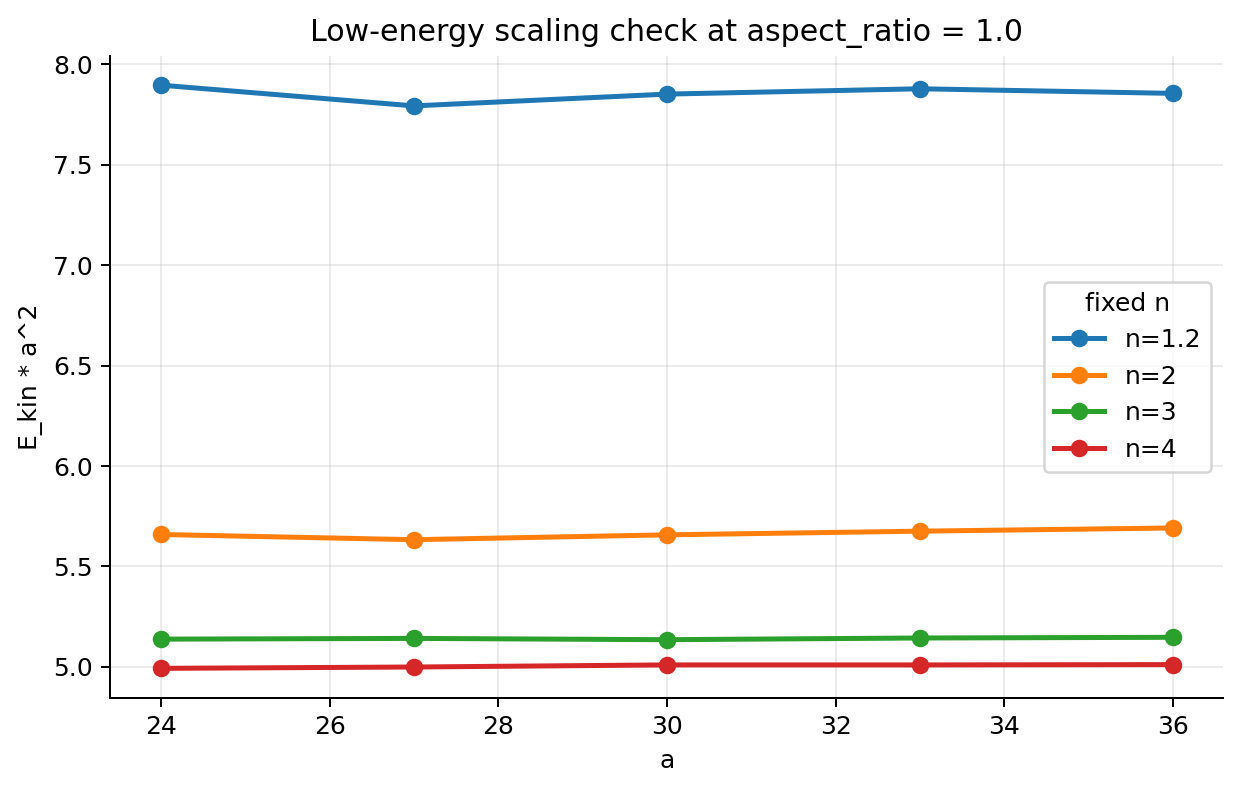
\includegraphics[width=0.85\textwidth]{../reports/assets/e0_kin_a2_scaling_by_n.png}
  \caption{TODO: Проверка масштабирования $(E_0 + 4)a^2$ для фиксированных $n$.}
\end{figure}

\section{Bessel sanity check для n = 2, aspect ratio = 1}
\todo{Bessel check at $a=36$ has about 2.03\% relative error.}

\begin{figure}[htbp]
  \centering
  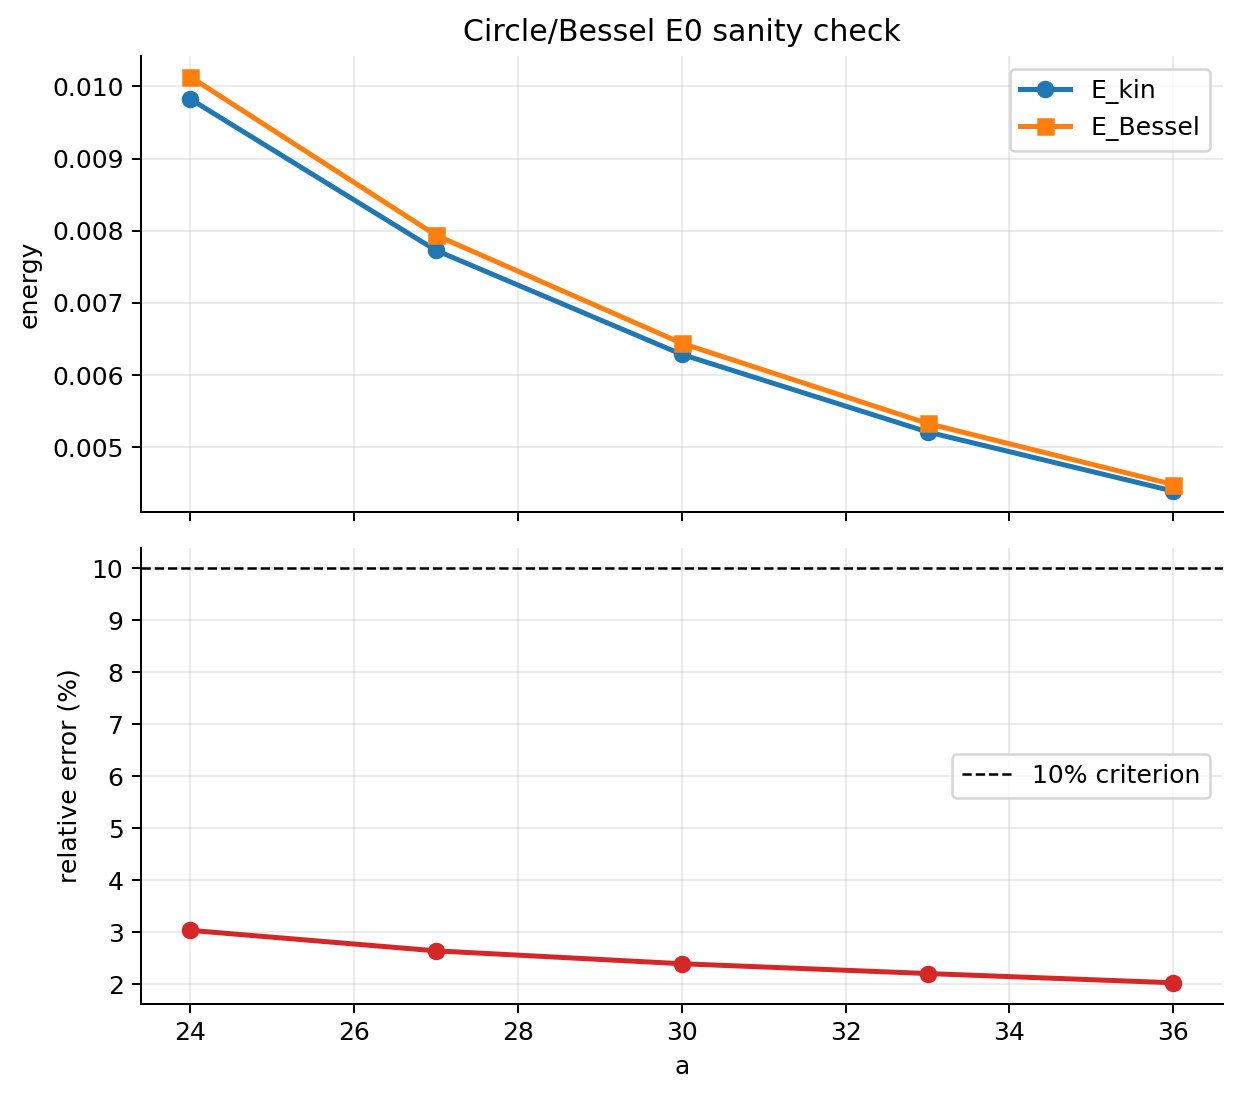
\includegraphics[width=0.85\textwidth]{../reports/assets/circle_bessel_e0_check.png}
  \caption{TODO: Bessel sanity check для кругового случая $n=2$, aspect ratio = 1.}
\end{figure}

\section{Вырождение уровней и исключение dE2 из основных целей}
\todo{$dE_2$ for $n=2$, aspect ratio = 1 is numerically zero across the inspected slice.}
\todo{Объяснить, почему это поддерживает diagnostic-only статус $dE_2$.}

\begin{figure}[htbp]
  \centering
  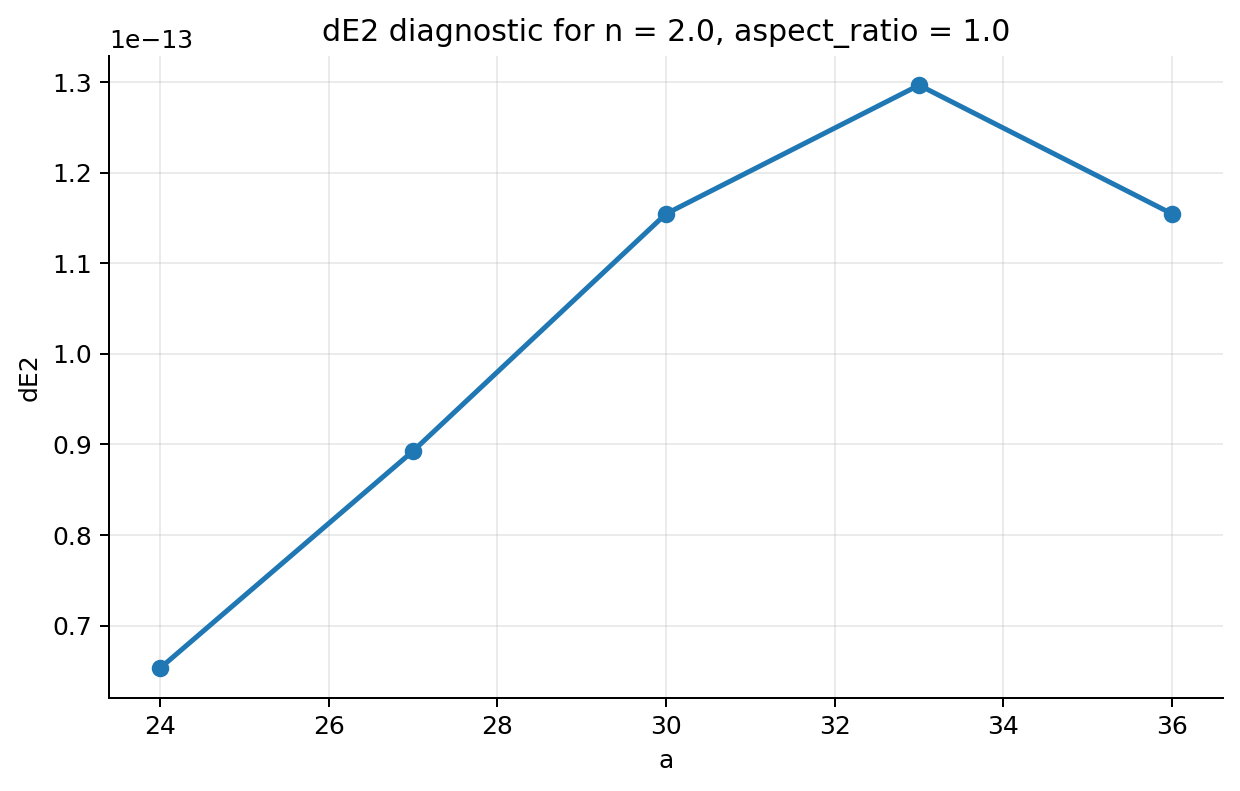
\includegraphics[width=0.80\textwidth]{../reports/assets/de2_near_degeneracy_n2_ar1.png}
  \caption{TODO: Диагностика near-degeneracy для $dE_2$ в круговом случае.}
\end{figure}

\section{Диагностики дискретизации границы}
\todo{$N_{\mathrm{sites}} / \mathrm{analytic\_area}$ ranges approximately from 0.98094 to 1.00761.}
\todo{max sublattice imbalance ratio about 2.16\%, largest at $n=1.2$, $a=24$, aspect ratio = 1.0.}

\begin{figure}[htbp]
  \centering
  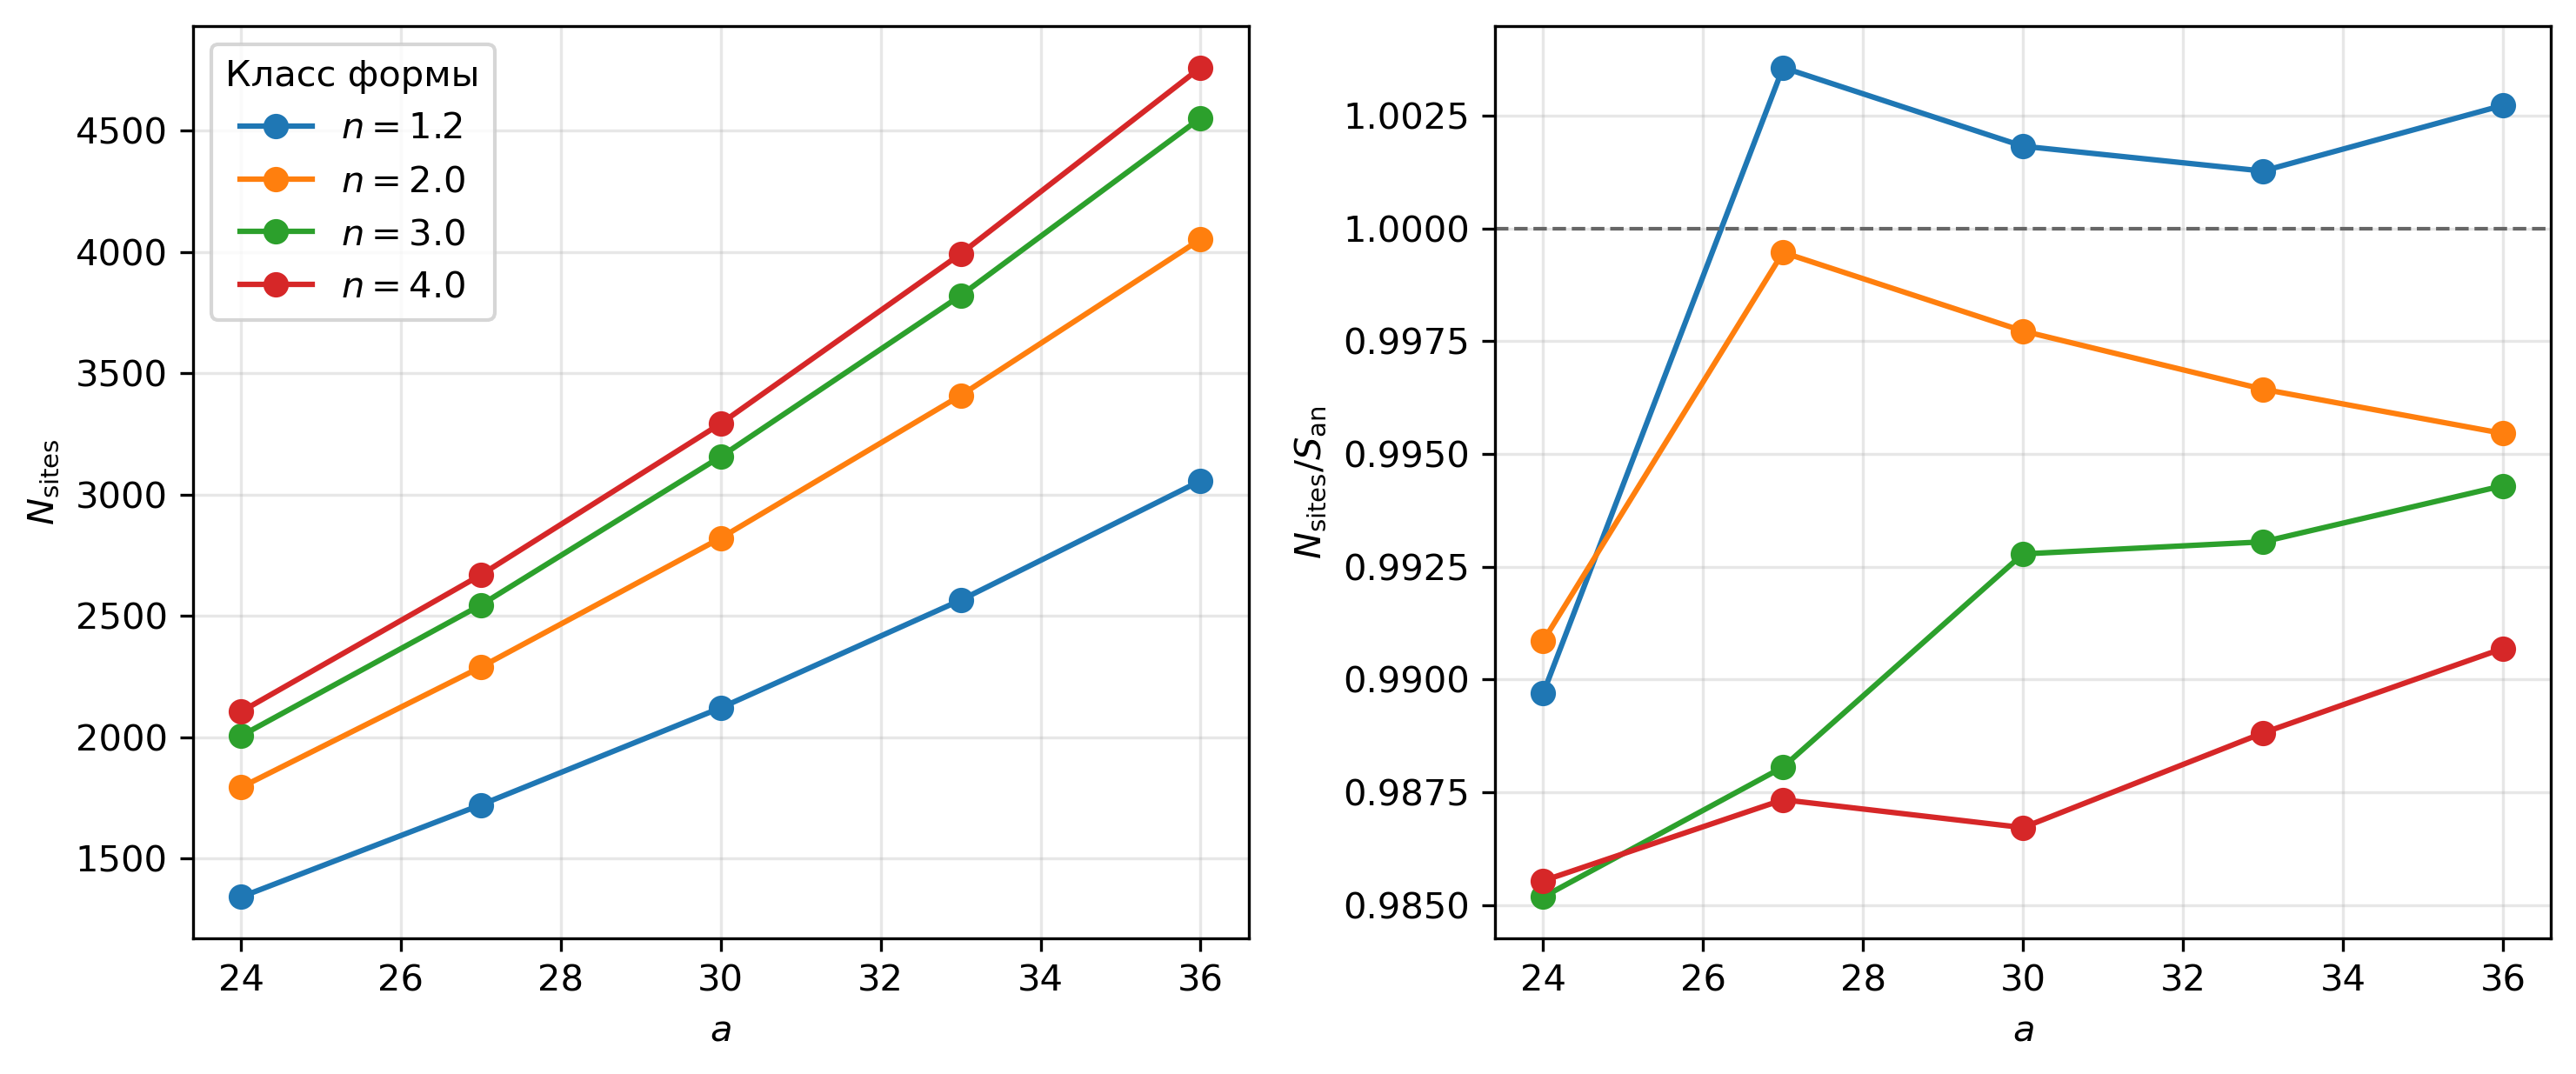
\includegraphics[width=0.85\textwidth]{../reports/assets/nsites_area_ratio_by_n.png}
  \caption{TODO: Сравнение числа узлов и аналитической площади.}
\end{figure}

\begin{figure}[htbp]
  \centering
  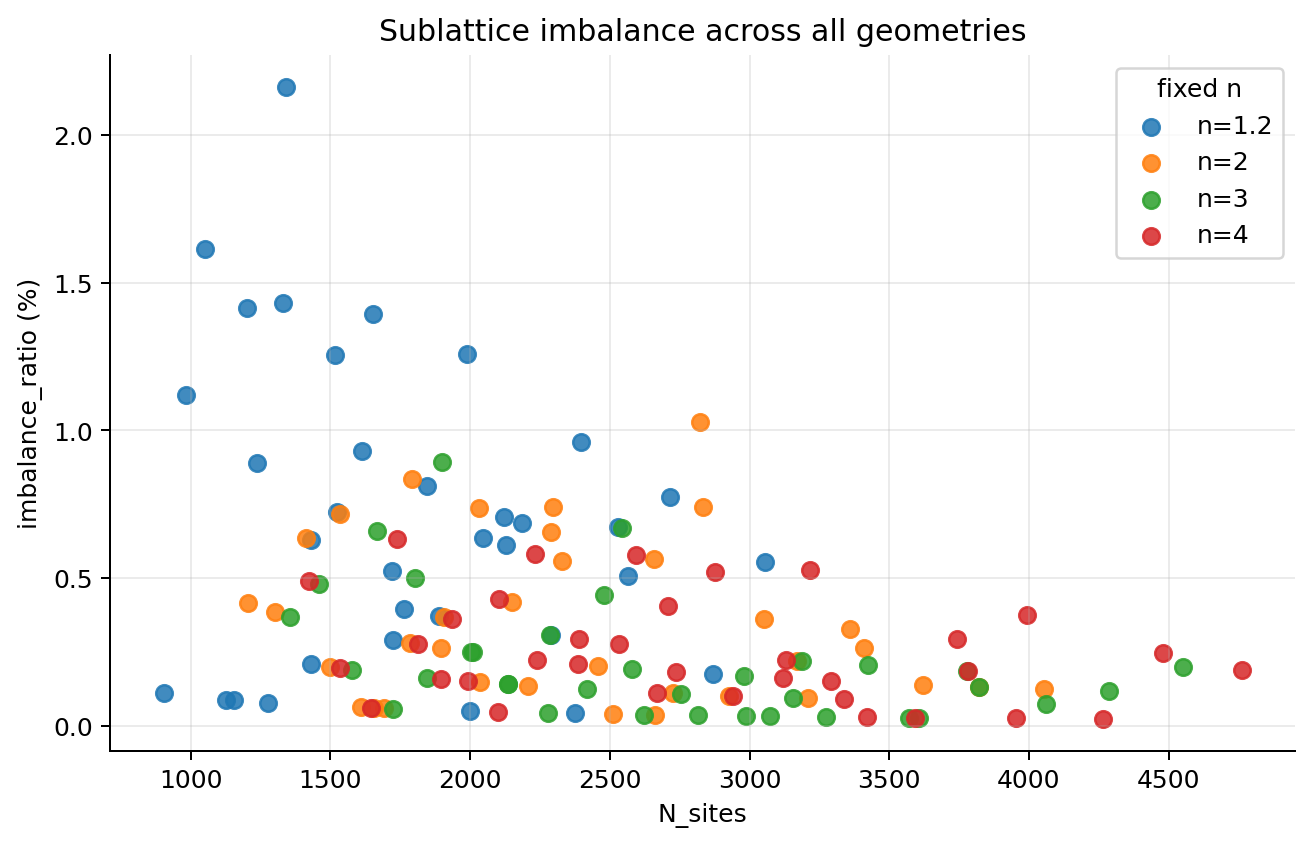
\includegraphics[width=0.85\textwidth]{../reports/assets/sublattice_imbalance_summary.png}
  \caption{TODO: Диагностика подрешёточного дисбаланса.}
\end{figure}

\section{Выводы по главе 3}
\todo{Сформулировать выводы: физический режим проверен, но это не доказательство continuum limit и не утверждение глобальной оптимальности признаков.}

\clearpage

\chapter{ФИЗИЧЕСКИ МОТИВИРОВАННАЯ СУРРОГАТНАЯ МОДЕЛЬ}

\section{Выбор признаков на основе scaling \texorpdfstring{$1/a^2$}{1/a^2}}

В предыдущей главе было показано, что для рассматриваемых суперэллиптических квантовых точек величина $E_{\mathrm{kin}}=E_0+4$ приблизительно масштабируется как $1/a^2$ в выбранном design window. Это согласуется с низкоэнергетическим квадратичным пределом square-lattice tight-binding модели, где характерное волновое число ограниченного состояния масштабируется как $k \sim 1/a$, а энергия, отсчитанная от дна зоны, как $k^2$.

Поэтому признаки суррогатной модели выбираются не путём слепого перебора, а из физической структуры задачи. Для фиксированного класса формы $n$ используются геометрические параметры $a$ и $r_{\mathrm{AR}}$, где $b=a r_{\mathrm{AR}}$. В анизотропном случае второе геометрическое направление также влияет на спектр, поэтому один только признак $1/a^2$ недостаточен для описания всей сетки параметров.

В качестве физически мотивированного набора признаков используется
\begin{equation}
  x_1 = \frac{1}{a^2}, \qquad
  x_2 = \frac{1}{a^2 r_{\mathrm{AR}}}, \qquad
  x_3 = r_{\mathrm{AR}} .
\end{equation}
Первый признак кодирует основной размерный масштаб, ожидаемый из низкоэнергетического закона $E_{\mathrm{kin}}\sim 1/a^2$. Второй признак является простой формой учёта второго геометрического масштаба, связанного с $b=a r_{\mathrm{AR}}$, и по смыслу близок к inverse-area-like зависимости. Третий признак оставляет в модели прямую информацию об анизотропии формы, которая может не полностью сводиться к степенным масштабам.

Такой выбор признаков не означает, что данный набор является единственным возможным или глобально оптимальным. Он означает только, что в проверенном диапазоне параметров признаки согласованы с физической картиной низкоэнергетического confinement и могут служить компактным описанием основной зависимости спектра от размера и формы. Обобщение за пределы диапазонов $a \in [24,36]$ и $r_{\mathrm{AR}} \in [0.67,1.0]$ в данной работе не утверждается.

Целевыми величинами для основной регрессии являются $E_0$ и $dE_1=E_1-E_0$. Величина $dE_2$ сохраняется как диагностическая, но не используется как основная цель суррогатной модели из-за чувствительности к вырождению и порядку уровней, описанной в главе 3.

\section{Ridge-регрессия как интерпретируемый baseline}

Основной baseline в работе построен на Ridge-регрессии. Это линейная модель в выбранном пространстве признаков:
\begin{equation}
  \hat{y}
  =
  \beta_0
  +
  \sum_{j=1}^{3} \beta_j x_j ,
\end{equation}
где $\hat{y}$ обозначает предсказание для $E_0$ или $dE_1$, а $x_j$ --- физически мотивированные признаки. Ridge-регрессия минимизирует ошибку с добавлением $L_2$-регуляризации коэффициентов:
\begin{equation}
  \mathcal{L}
  =
  \sum_i \left(y_i-\hat{y}_i\right)^2
  +
  \alpha \sum_j \beta_j^2 .
\end{equation}

Такой baseline не является формальной игрушечной моделью. Для малых структурированных датасетов низкая ёмкость модели является преимуществом: она снижает риск подгонки к отдельным точкам сетки и делает результат устойчивее к небольшим lattice-эффектам. $L_2$-регуляризация стабилизирует коэффициенты, а линейность в физически выбранных признаках облегчает интерпретацию. Если такая модель хорошо аппроксимирует спектральную характеристику, это означает, что существенная часть зависимости уже описывается проверенным scaling и простой анизотропной поправкой.

Перед обучением признаки стандартизируются, чтобы регуляризация действовала сопоставимо на разные компоненты признакового вектора. При этом метрики качества вычисляются в исходных физических единицах hopping-параметра $t$, а не в нормированных единицах. Параметры baseline фиксируются заранее; tuning гиперпараметров не используется как дополнительный способ улучшить результат после просмотра тестовых ошибок.

В данной методологии Ridge остаётся предпочтительной моделью по умолчанию, пока более сложная модель не демонстрирует устойчивого и заранее определённого преимущества. Такой подход соответствует физической задаче: цель состоит не в максимизации сложности surrogate-модели, а в получении проверяемой аппроксимации спектра модельной наноструктуры.

\section{Протоколы структурированной валидации LOAO и LOARO}

Обычное случайное разбиение train/test не является подходящим основным протоколом для данного датасета. Геометрии образуют регулярную параметрическую сетку по $a$ и $r_{\mathrm{AR}}$, поэтому при random split в обучающей и тестовой выборках с высокой вероятностью оказываются соседние точки сетки. Такая проверка может завышать качество, поскольку фактически оценивает локальную интерполяцию между близкими геометриями, а не устойчивость модели к исключению целого значения физического параметра. Для структурированных пространственных и параметрических данных необходимость более строгих схем валидации также обсуждается в литературе по structured cross-validation~\cite{roberts2017crossvalidation}.

Поэтому сравнение моделей проводится отдельно внутри каждого фиксированного класса $n$ с использованием двух протоколов. Первый протокол, LOAO, означает leave-one-$a$-out. Для каждого значения $a$ все геометрии с этим размером исключаются из обучения и используются как тестовая fold-группа:
\[
  \mathcal{D}_{\mathrm{test}}(a^\ast)
  =
  \{(a,r_{\mathrm{AR}}): a=a^\ast\}.
\]
Остальные значения $a$ образуют обучающую выборку. Такой протокол проверяет обобщение на невиданные значения размера внутри фиксированного класса формы.

Второй протокол, LOARO, означает leave-one-aspect-ratio-out. Для каждого значения $r_{\mathrm{AR}}$ из обучения исключаются все геометрии с данным отношением сторон:
\[
  \mathcal{D}_{\mathrm{test}}(r_{\mathrm{AR}}^\ast)
  =
  \{(a,r_{\mathrm{AR}}): r_{\mathrm{AR}}=r_{\mathrm{AR}}^\ast\}.
\]
Такой протокол проверяет обобщение на невиданные aspect ratios при сохранении фиксированного набора размеров.

Основной метрикой сравнения является MAE:
\begin{equation}
  \mathrm{MAE}
  =
  \frac{1}{M}
  \sum_{i=1}^{M}
  \left|\hat{y}_i-y_i\right| .
\end{equation}
Она вычисляется в физических единицах $t$. Это важно, поскольку суррогатная модель может использовать внутреннее масштабирование признаков или цели, но итоговая ошибка должна характеризовать реальную ошибку аппроксимации спектральной величины.

\section{Tiny MLP ablation}

Нелинейная модель в этой работе используется только как ablation/control experiment. Её задача --- проверить, даёт ли малая нелинейность устойчивое преимущество по сравнению с physics-informed Ridge при тех же структурированных протоколах валидации. MLP не рассматривается как источник физических законов и не заменяет прямой расчёт спектра в Kwant.

Используется намеренно малая архитектура. Для каждого фиксированного $n$ доступно только 35 точек параметрической сетки: пять значений $a$ и семь значений $r_{\mathrm{AR}}$. В таких условиях большая нейронная сеть легко может начать подгонять особенности конкретных fold-разбиений, особенно при наличии lattice-эффектов и малых зазоров между уровнями. Поэтому hidden layer состоит только из четырёх нейронов:
\[
  \texttt{hidden\_layer\_sizes=(4,)}.
\]
Вопрос о минимально необходимом объёме данных отдельно не исследовался, поэтому из результатов не делается утверждение о data efficiency.

Конфигурация tiny MLP фиксируется заранее:
\begin{itemize}
  \item внешний estimator: \texttt{TransformedTargetRegressor};
  \item масштабирование цели: \texttt{StandardScaler};
  \item regressor: \texttt{Pipeline};
  \item масштабирование признаков: \texttt{("scale", StandardScaler())};
  \item внутренняя модель: \texttt{MLPRegressor};
  \item \texttt{hidden\_layer\_sizes=(4,)};
  \item \texttt{activation="tanh"};
  \item \texttt{solver="lbfgs"};
  \item \texttt{alpha=1e-3};
  \item \texttt{early\_stopping=False};
  \item \texttt{random\_state=42} для фиксированной конфигурации;
  \item \texttt{max\_iter=5000}.
\end{itemize}

Для MLP рассматриваются два варианта признаков. Вариант MLP+raw использует исходные геометрические параметры $a$ и $r_{\mathrm{AR}}$. Вариант MLP+physics использует тот же physics-informed набор признаков, что и Ridge. Это разделение позволяет проверить две разные вещи: полезна ли малая нелинейность сама по себе и сохраняется ли преимущество физических признаков при нелинейной модели.

Поскольку обучение MLP может зависеть от начального состояния оптимизации, для оценки устойчивости используются несколько значений \texttt{random\_state}. Кроме того, для каждого fold фиксируется число итераций оптимизатора. Если модель достигает \texttt{max\_iter}, такой случай считается convergence failure и не может служить основанием для признания MLP устойчиво лучшей моделью.

\section{Предрегистрация критериев сравнения моделей}

Критерии сравнения Ridge и tiny MLP были зафиксированы до анализа результатов. Это необходимо, чтобы избежать post-hoc выбора модели по наиболее выгодным срезам таблицы ошибок. Сравнение проводится по ячейкам, определяемым тройкой:
\[
  (n,\; \mathrm{target},\; \mathrm{protocol}),
\]
где $n \in \{1.2,2.0,3.0,4.0\}$, target $\in \{E_0,dE_1\}$, а protocol $\in \{\mathrm{LOAO},\mathrm{LOARO}\}$. Всего получается
\[
  4 \times 2 \times 2 = 16
\]
основных comparison cells.

MLP+physics может считаться предпочтительной моделью только при устойчивом улучшении относительно Ridge+physics. Улучшение в каждой ячейке измеряется по MAE:
\begin{equation}
  \Delta_{\mathrm{MAE}}
  =
  \mathrm{MAE}_{\mathrm{Ridge}}
  -
  \overline{\mathrm{MAE}}_{\mathrm{MLP}},
\end{equation}
где среднее для MLP берётся по 10 значениям random seed. Относительное улучшение должно составлять не менее 15\%:
\begin{equation}
  \frac{\Delta_{\mathrm{MAE}}}{\mathrm{MAE}_{\mathrm{Ridge}}}
  \geq 0.15 .
\end{equation}
Порог 15\% выбран как консервативный практический минимум: меньшие отличия на малом структурированном датасете трудно отделить от fold-variability, seed-variability и дискретизационных эффектов границы.

Дополнительно проверяется seed stability. Для 10 запусков MLP определяется стандартная ошибка среднего:
\begin{equation}
  \mathrm{SE}
  =
  \frac{\mathrm{std}(\mathrm{MAE}_{\mathrm{MLP}})}{\sqrt{10}} .
\end{equation}
Улучшение считается устойчивым только если
\begin{equation}
  \Delta_{\mathrm{MAE}} > 0
  \quad \mathrm{and} \quad
  \Delta_{\mathrm{MAE}} > 2\,\mathrm{SE}.
\end{equation}
Таким образом, модель, которая в среднем хуже Ridge, не может быть признана стабильной даже при большой вариативности по seed.

Наконец, используется правило сходимости: если в данной comparison cell хотя бы один MLP+physics fit достигает \texttt{max\_iter}, эта ячейка не засчитывается как success независимо от значения MAE. Это правило предотвращает ситуацию, когда численно нестабильный результат интерпретируется как физически или статистически устойчивое улучшение.

Полное предпочтение MLP возможно только при выполнении критерия не только в сумме по всем 16 ячейкам, но и отдельно для обоих протоколов. Успех только в LOAO или только в LOARO рассматривается как частичное наблюдение, но не как основание заменить Ridge в качестве основной модели. Если предзарегистрированный критерий не выполняется, Ridge остаётся предпочтительной моделью благодаря простоте, интерпретируемости, стабильности и физической мотивированности признаков. Итог этого сравнения анализируется в главе 5.

\section{Выводы по главе 4}

В данной главе сформулирована методология суррогатного моделирования низкоэнергетического спектра модельных суперэллиптических квантовых точек. Основные выводы состоят в следующем.

\begin{enumerate}
  \item Набор признаков $\{1/a^2,\;1/(a^2 r_{\mathrm{AR}}),\;r_{\mathrm{AR}}\}$ выбран из физической картины низкоэнергетического scaling, подтверждённой в главе 3.
  \item Ridge-регрессия является основной интерпретируемой baseline-моделью: она линейна в физически мотивированных признаках, имеет малую ёмкость и стабилизируется $L_2$-регуляризацией.
  \item Случайное train/test-разбиение не используется как основной протокол, поскольку датасет является структурированной сеткой параметров. Вместо этого применяются LOAO и LOARO.
  \item Tiny MLP рассматривается только как контролируемая нелинейная ablation-модель, а не как источник физических законов или замена прямого Kwant-расчёта.
  \item Критерии сравнения моделей предзарегистрированы: учитываются порог улучшения MAE, устойчивость по seed, отсутствие convergence failures и выполнение требований отдельно для LOAO и LOARO.
  \item Численные результаты сравнения Ridge и tiny MLP рассматриваются в главе 5, где проверяется, выполняется ли предзарегистрированный критерий.
\end{enumerate}

\clearpage

\chapter{РЕЗУЛЬТАТЫ И ОБСУЖДЕНИЕ}

\section{Результаты физических sanity checks}
\todo{Свести результаты шага 07: energy convention, scaling, Bessel check, diagnostic-only status of $dE_2$.}

\section{Результаты physics-informed Ridge baseline}
\todo{Описать результаты Milestone 06c: Ridge как основной интерпретируемый baseline.}
\todo{Добавить таблицы MAE/RMSE после финальной подготовки текста.}

\section{Сравнение Ridge и tiny MLP}
\todo{MLP+physics succeeds in 10/16 cells overall.}
\todo{LOAO: 3/8.}
\todo{LOARO: 7/8.}
\todo{Criterion not met.}
\todo{Ridge remains preferred.}
\todo{LOAO failure concentrated in $dE_1$: all four n-classes have negative improvement for $dE_1$ under LOAO.}
\todo{For $E_0$ under LOAO, MLP improves in 3/4 n-classes.}
\todo{Conclusion: tiny MLP can add weak nonlinear corrections in some cases but does not robustly improve generalization to unseen size values for $dE_1$.}

\begin{figure}[htbp]
  \centering
  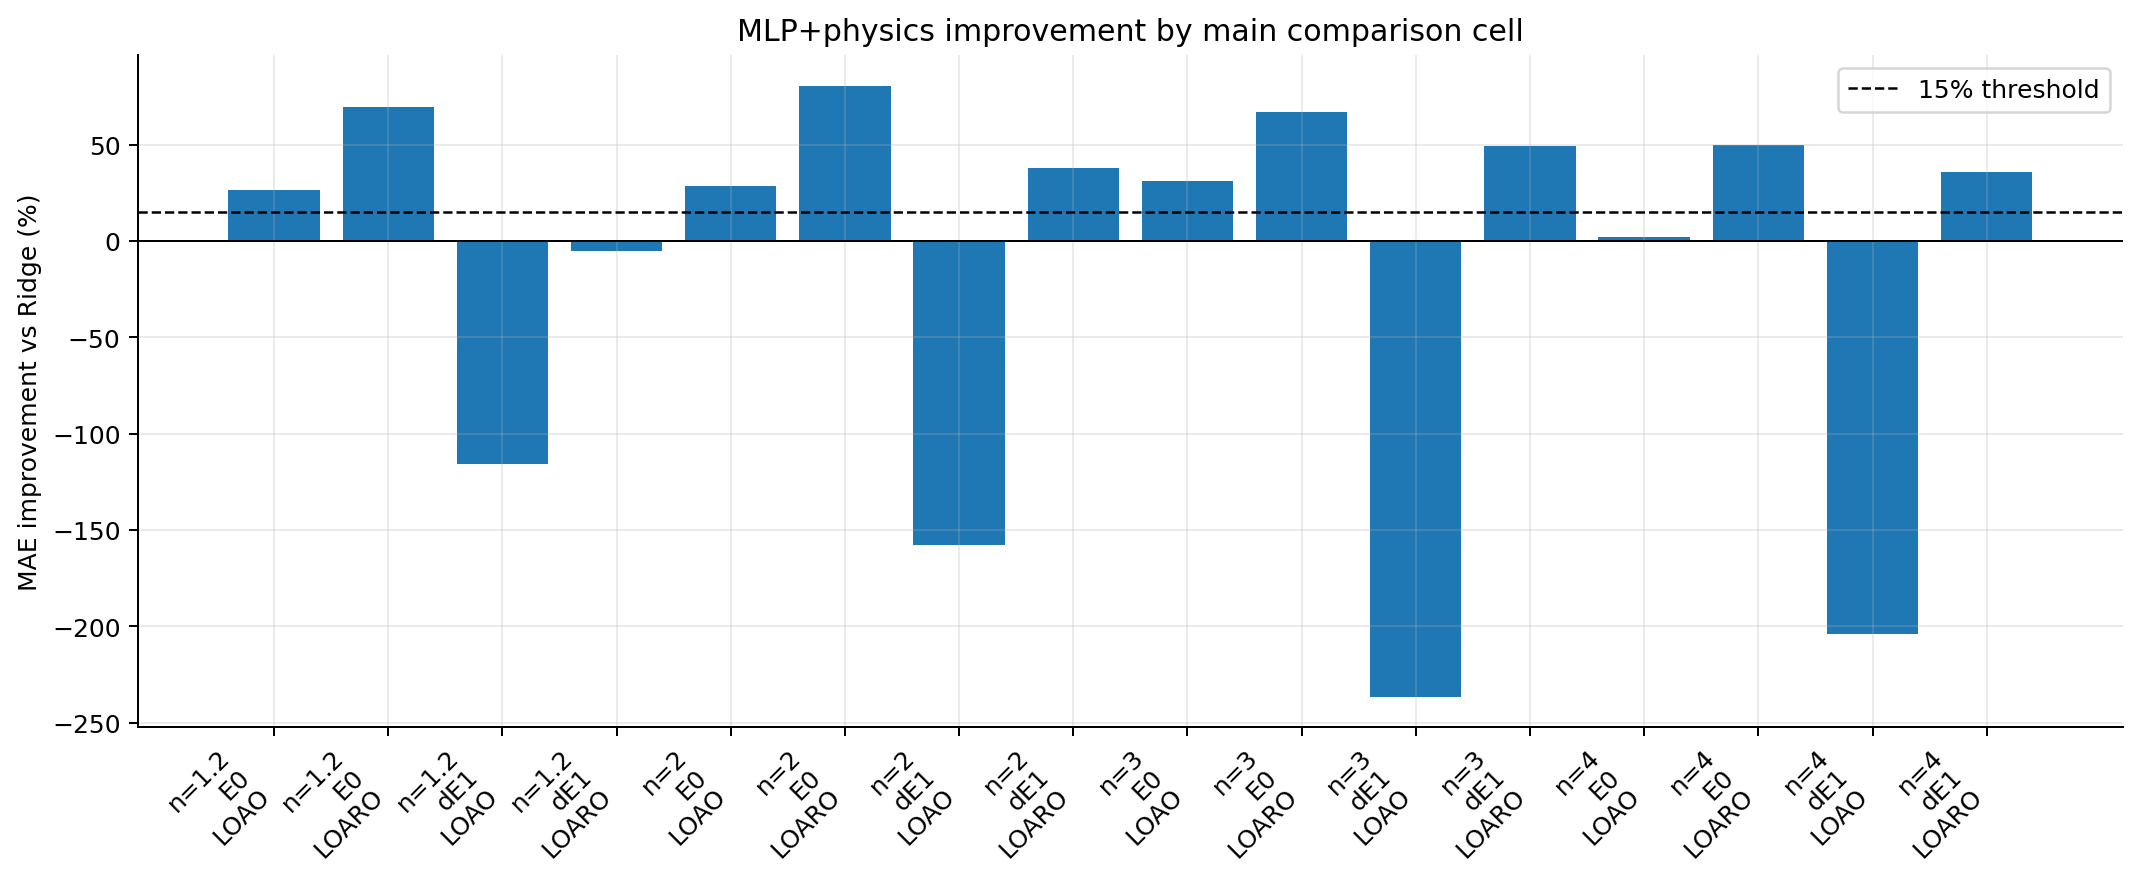
\includegraphics[width=0.85\textwidth]{../reports/assets/mlp_ablation_improvement_by_cell.png}
  \caption{TODO: Улучшение tiny MLP относительно Ridge по предрегистрационным ячейкам.}
\end{figure}

\begin{figure}[htbp]
  \centering
  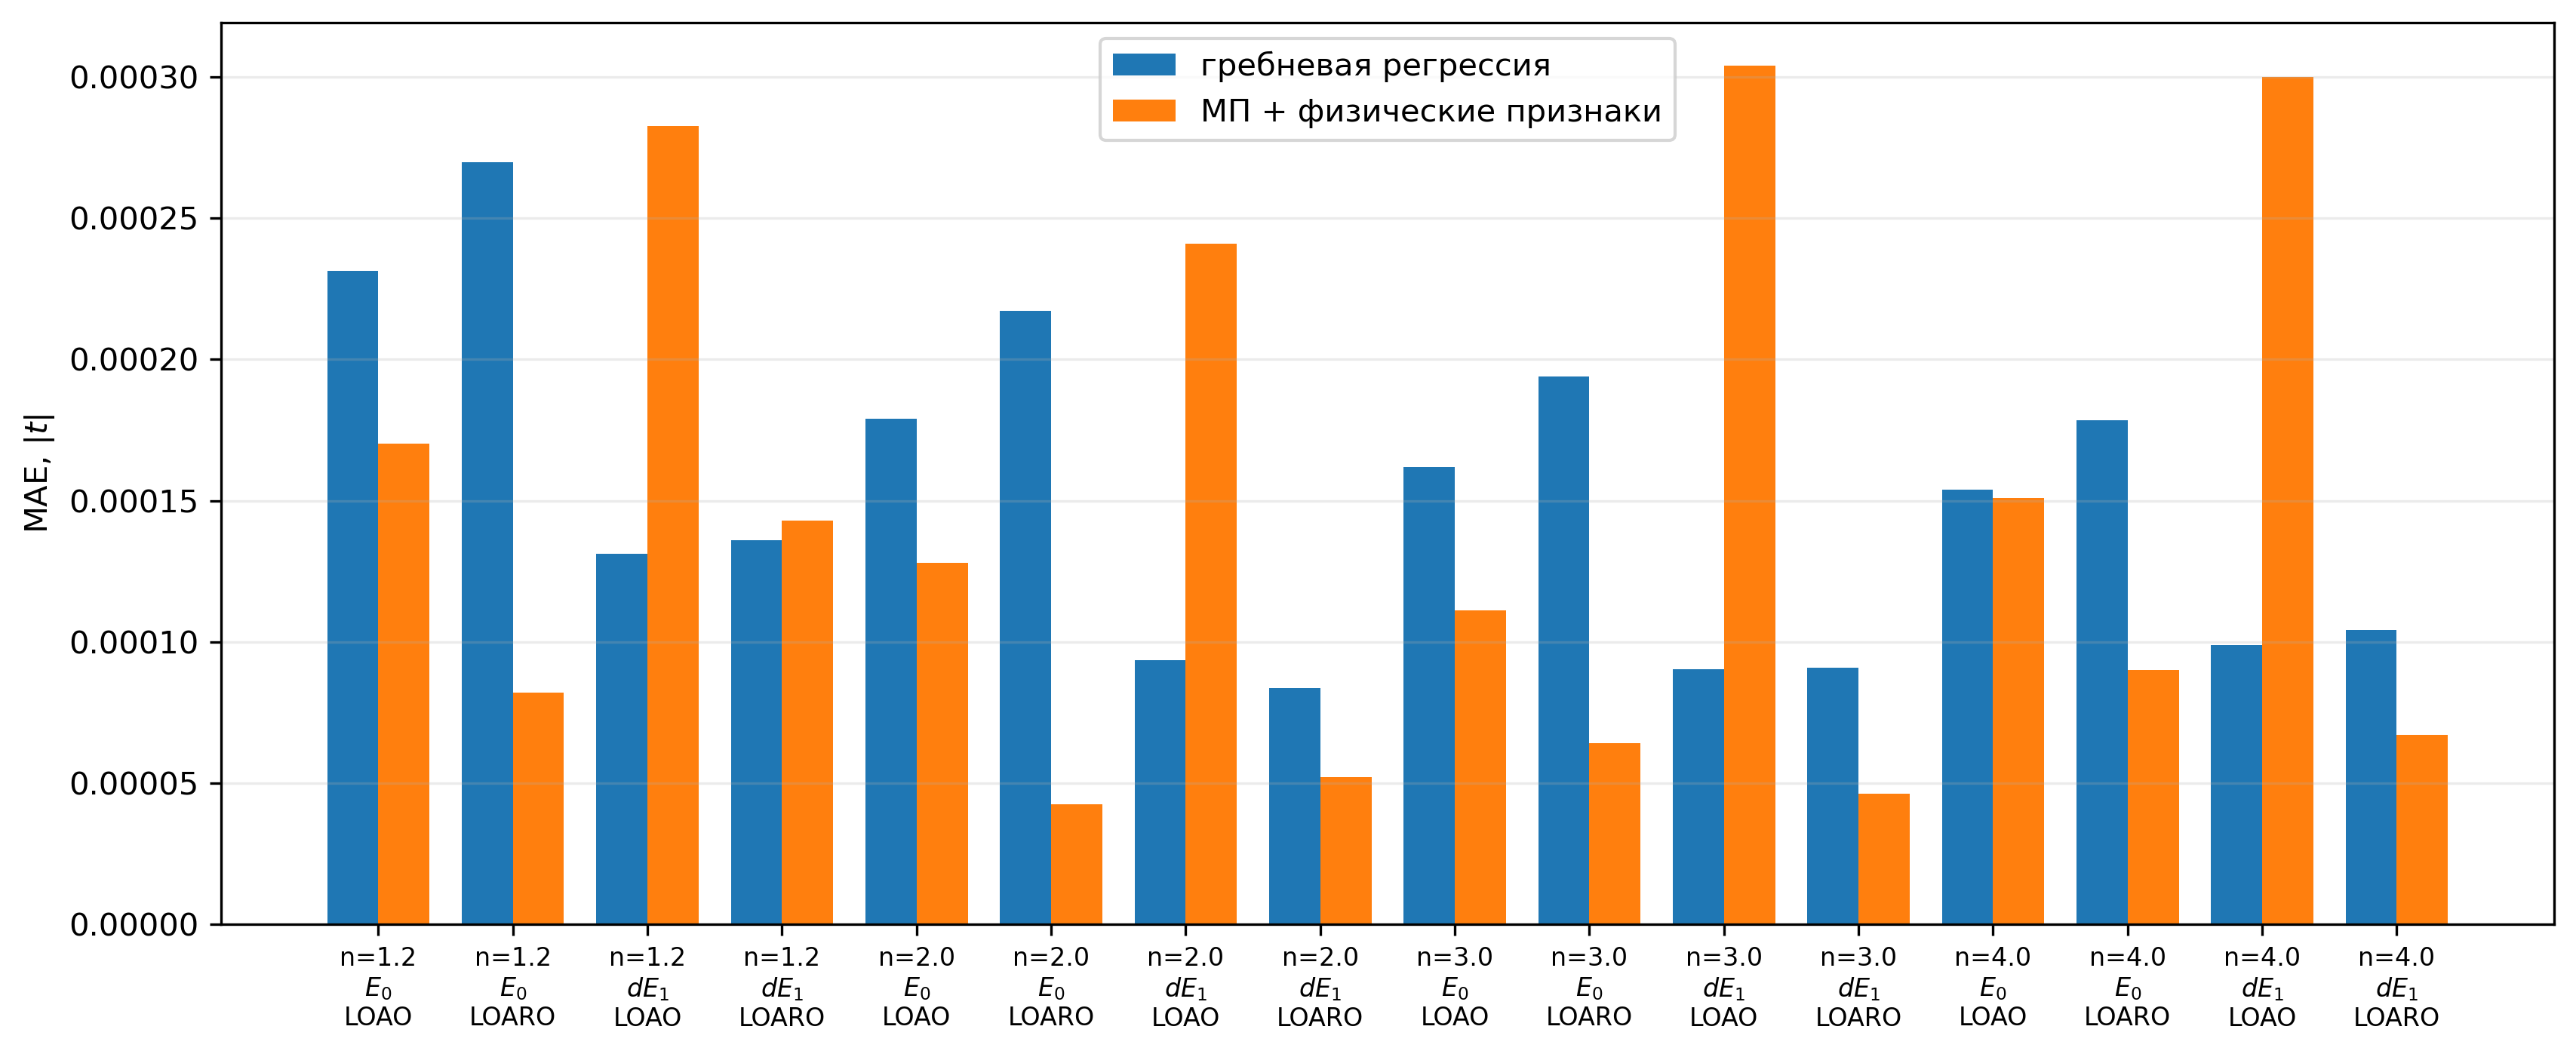
\includegraphics[width=0.85\textwidth]{../reports/assets/mlp_ablation_ridge_vs_mlp_physics_mae.png}
  \caption{TODO: Сравнение MAE Ridge и MLP+physics.}
\end{figure}

\begin{figure}[htbp]
  \centering
  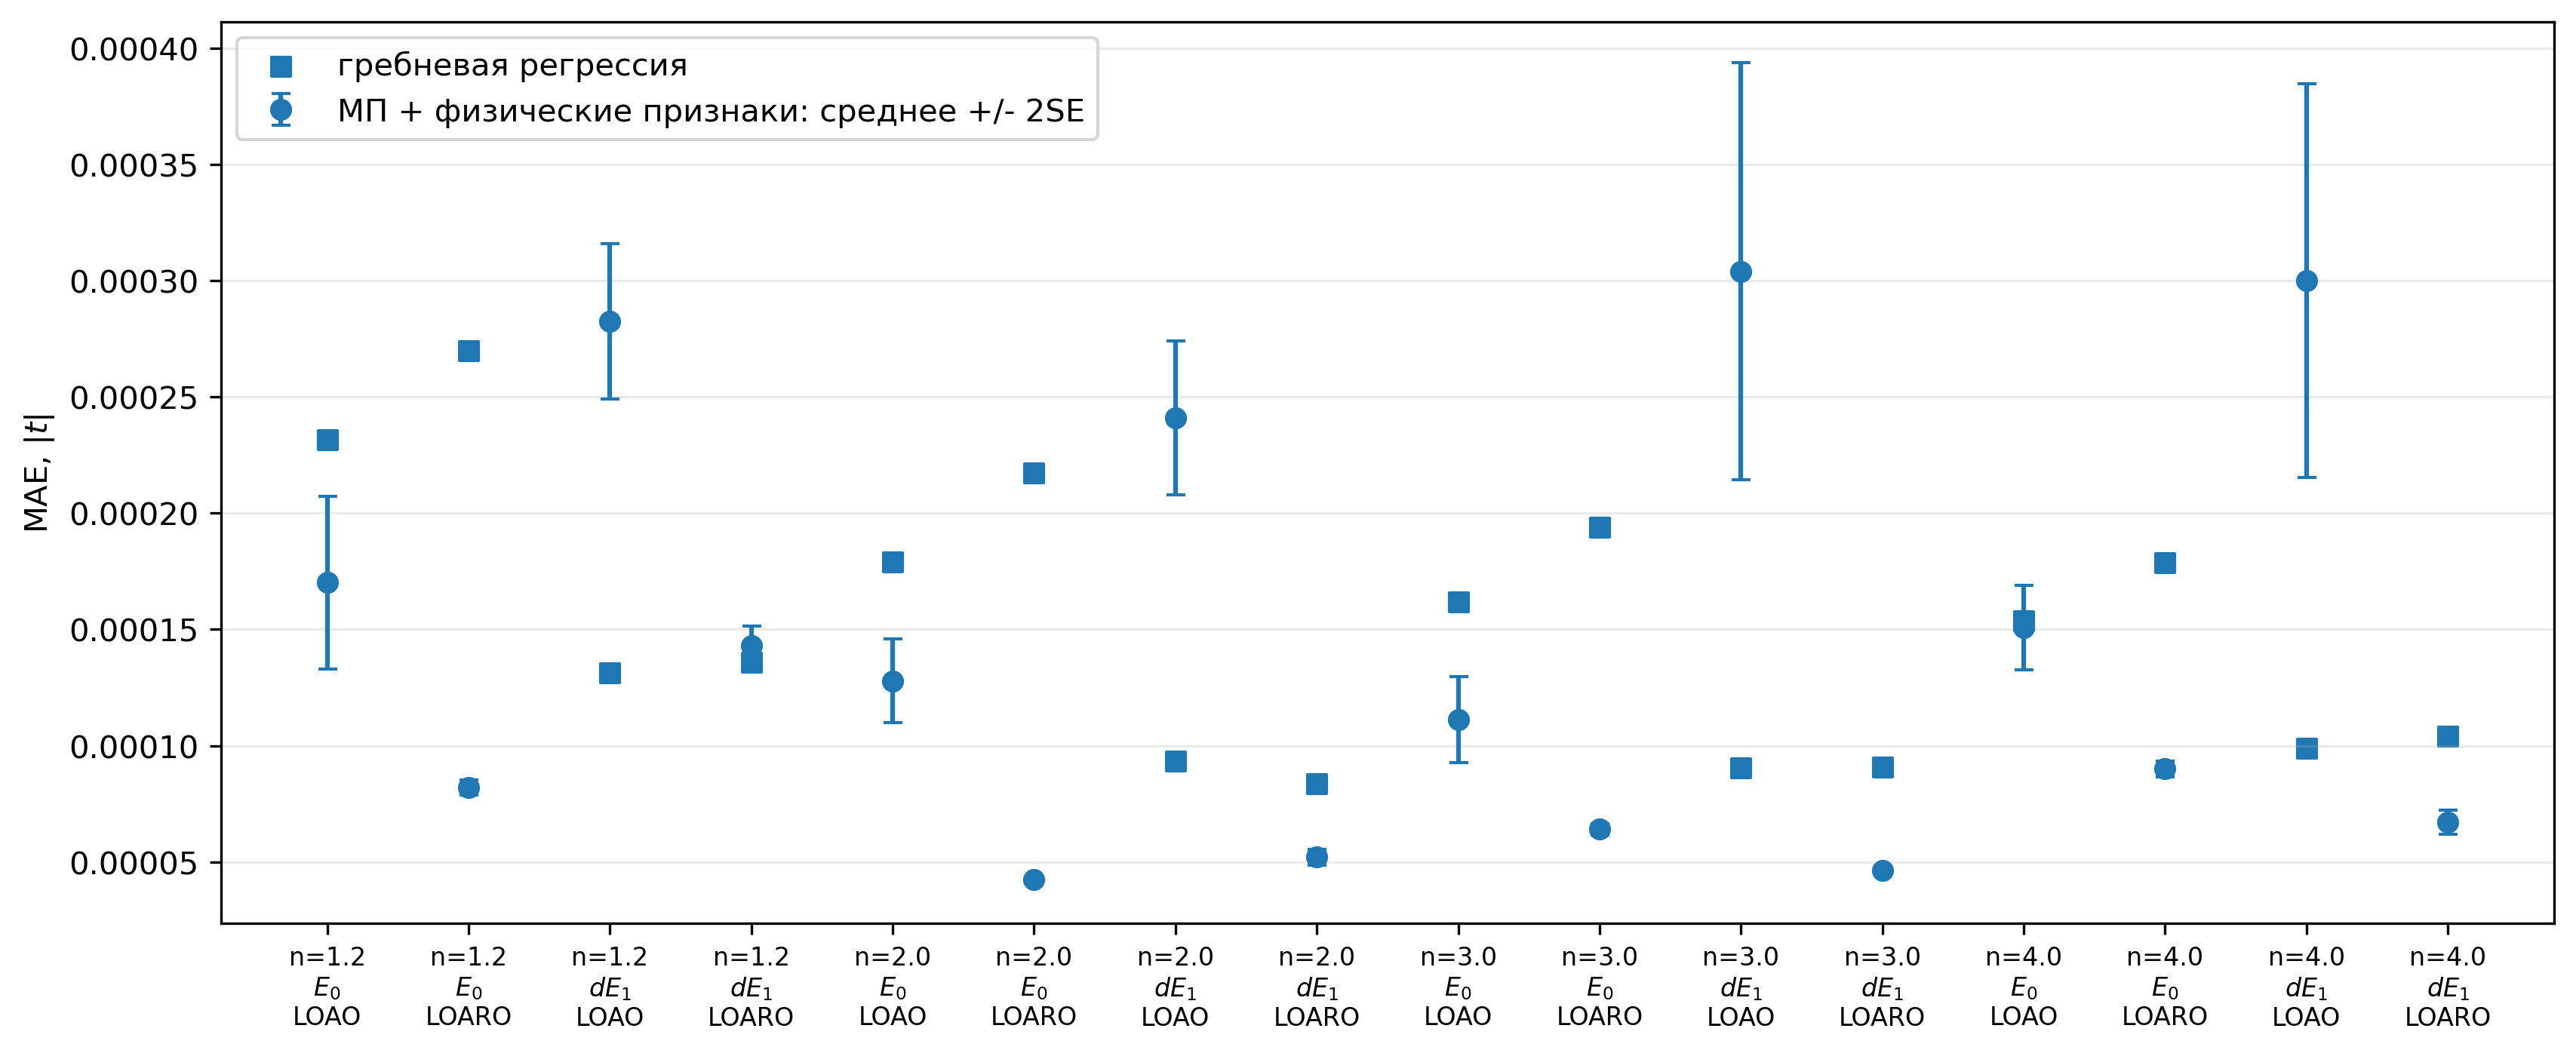
\includegraphics[width=0.85\textwidth]{../reports/assets/mlp_ablation_seed_stability.png}
  \caption{TODO: Устойчивость MLP+physics по random seeds.}
\end{figure}

\begin{figure}[htbp]
  \centering
  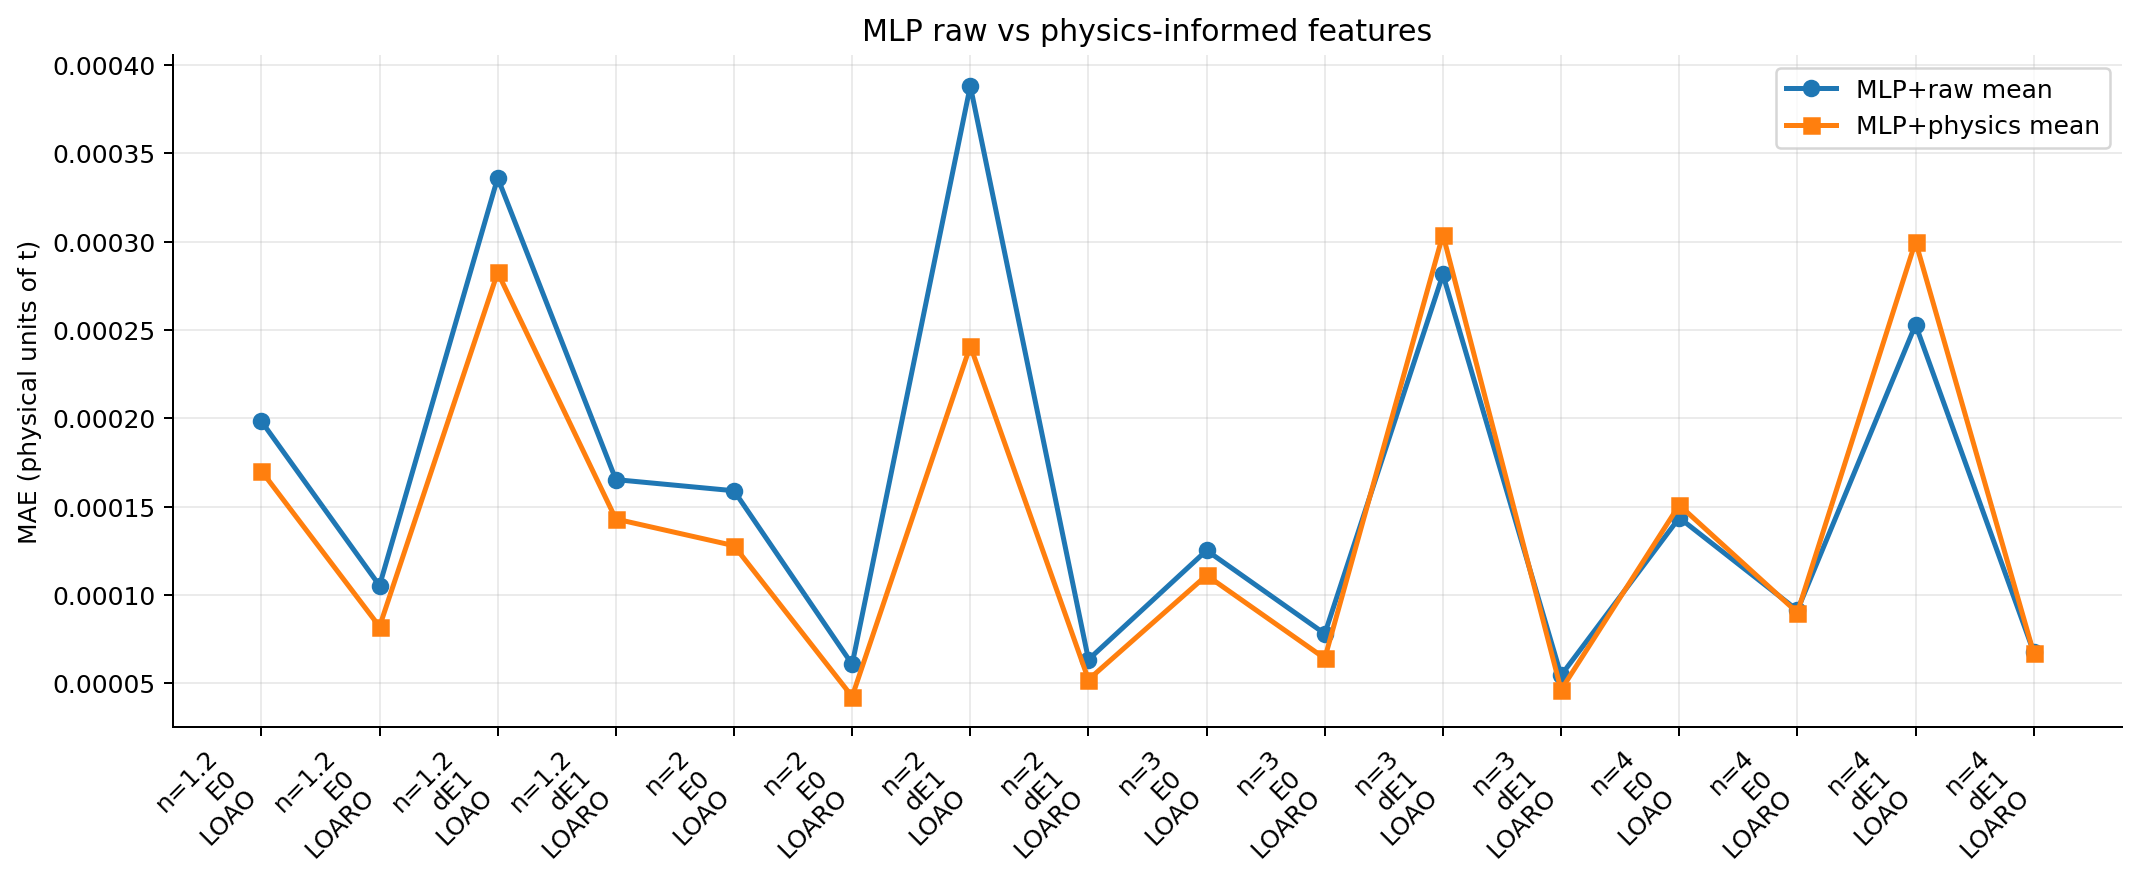
\includegraphics[width=0.85\textwidth]{../reports/assets/mlp_raw_vs_physics_features.png}
  \caption{TODO: Сравнение raw и physics-informed признаков для MLP.}
\end{figure}

\section{Анализ остатков Ridge}
\todo{Primary residual hypothesis not supported.}
\todo{Discretization dominated smooth macro-parameters in 3/4 n-classes.}
\todo{Meaningful discretization support only in 1/4 n-classes.}
\todo{Meaningful case: $n=1.2$, \texttt{imbalance\_ratio}, $\rho \approx 0.416$, $p \approx 0.013$.}
\todo{For $n \geq 2$, selected simple edge-discretization diagnostics do not systematically explain the remaining Ridge residuals.}
\todo{Mention that \texttt{imbalance\_ratio} and \texttt{abs\_delta\_N\_over\_N} are identical aliases if this is reflected in final step-09 cleanup.}

\begin{figure}[htbp]
  \centering
  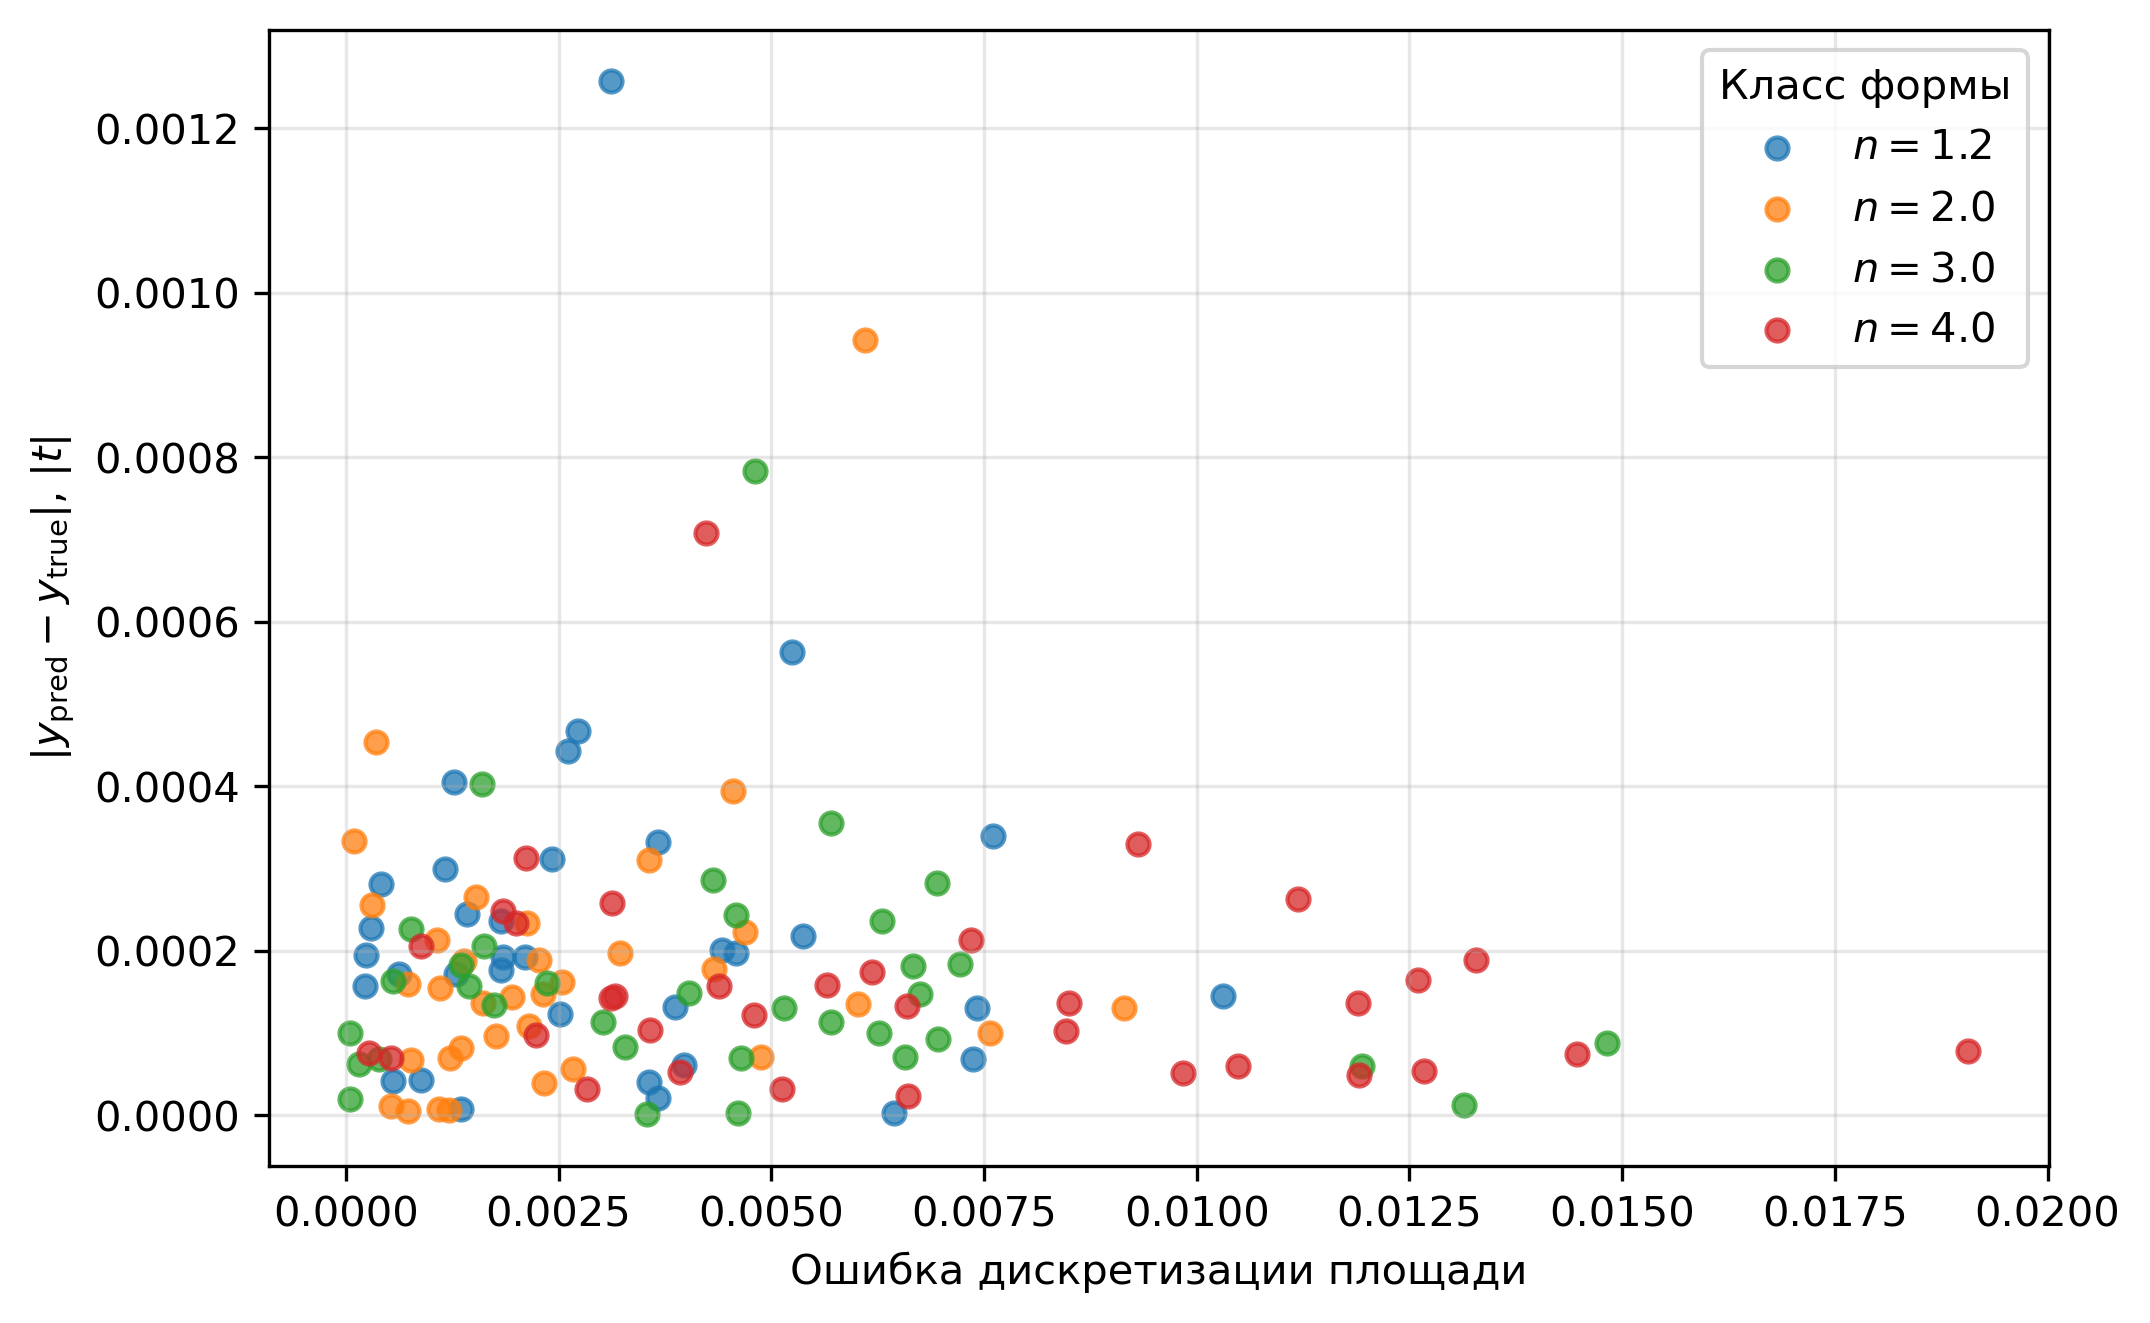
\includegraphics[width=0.85\textwidth]{../reports/assets/ridge_e0_loao_abs_residual_vs_edge_error.png}
  \caption{TODO: Остатки Ridge и ошибка дискретизации площади для E0/LOAO.}
\end{figure}

\begin{figure}[htbp]
  \centering
  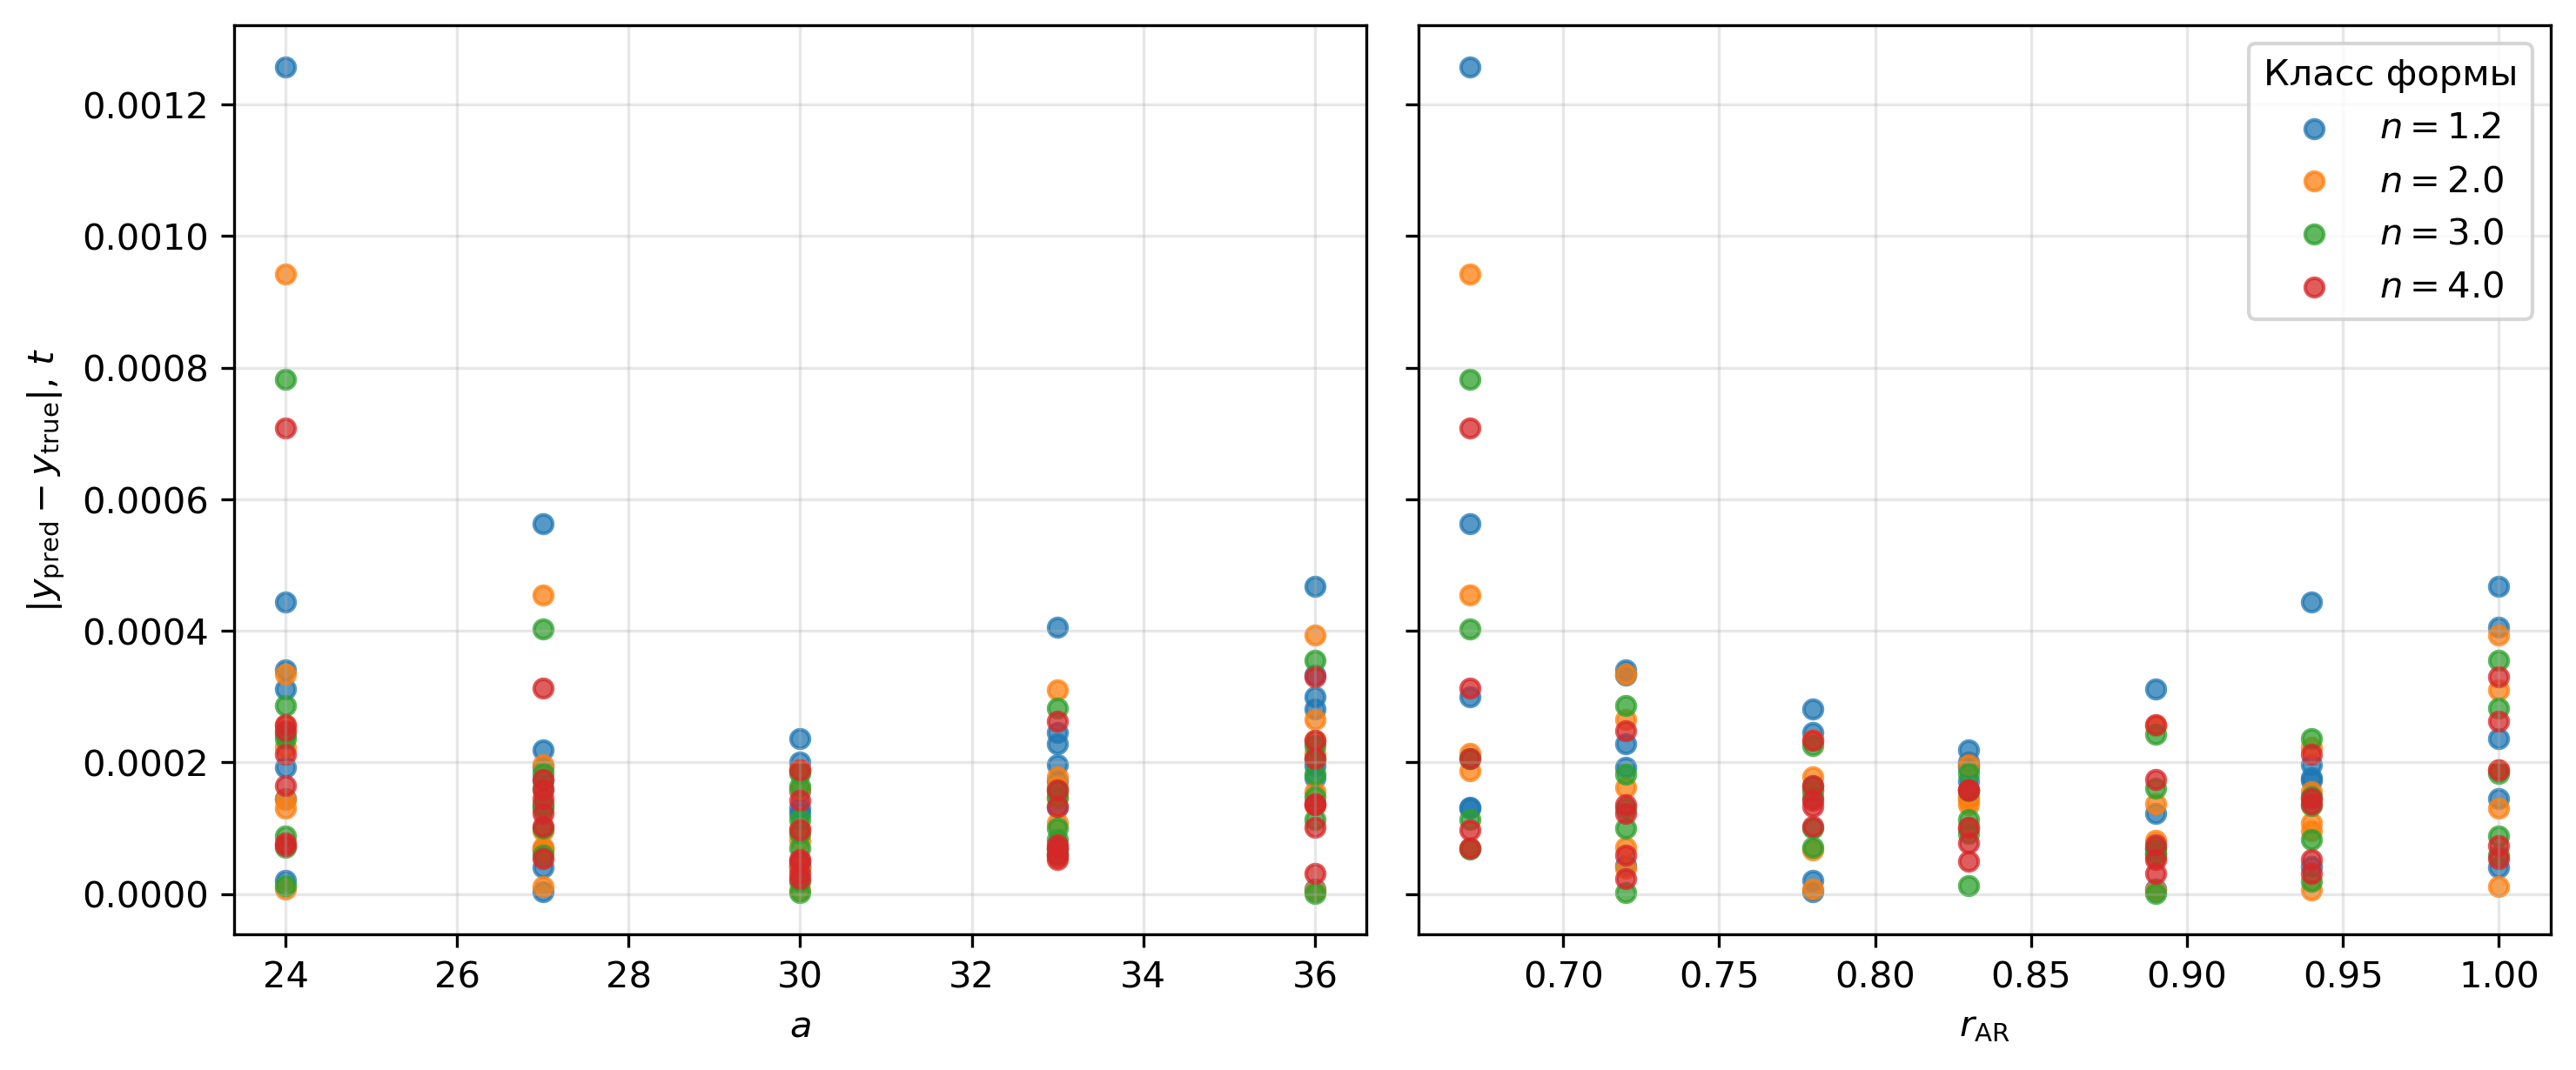
\includegraphics[width=0.85\textwidth]{../reports/assets/ridge_e0_loao_abs_residual_vs_macro_params.png}
  \caption{TODO: Остатки Ridge и гладкие макропараметры для E0/LOAO.}
\end{figure}

\begin{figure}[htbp]
  \centering
  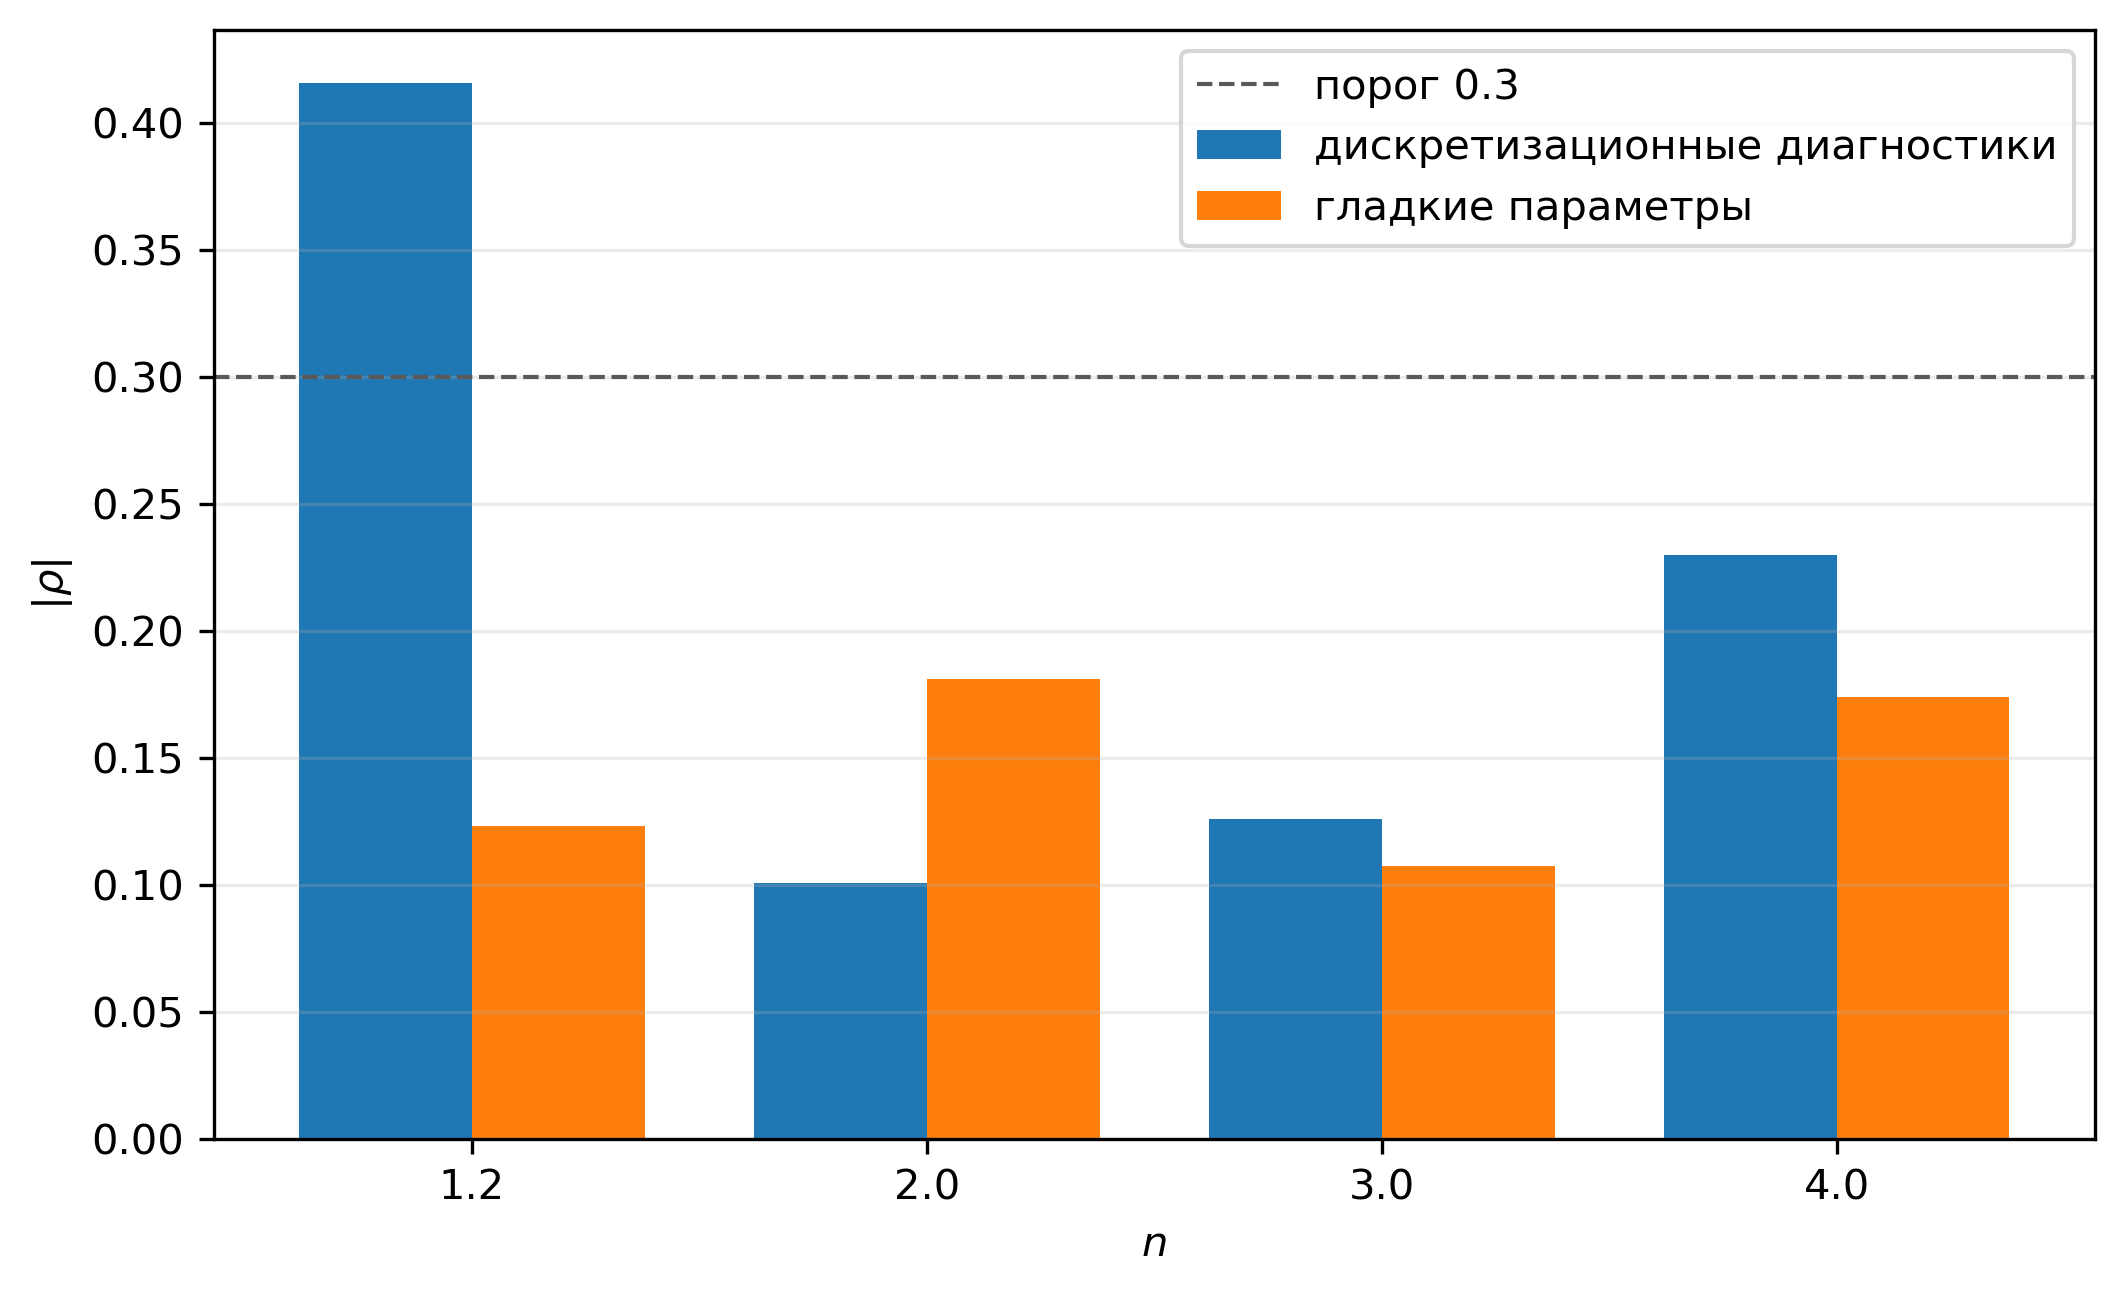
\includegraphics[width=0.85\textwidth]{../reports/assets/ridge_residual_dominance_by_n.png}
  \caption{TODO: Сравнение максимальных Spearman-корреляций по классам $n$.}
\end{figure}

\begin{figure}[htbp]
  \centering
  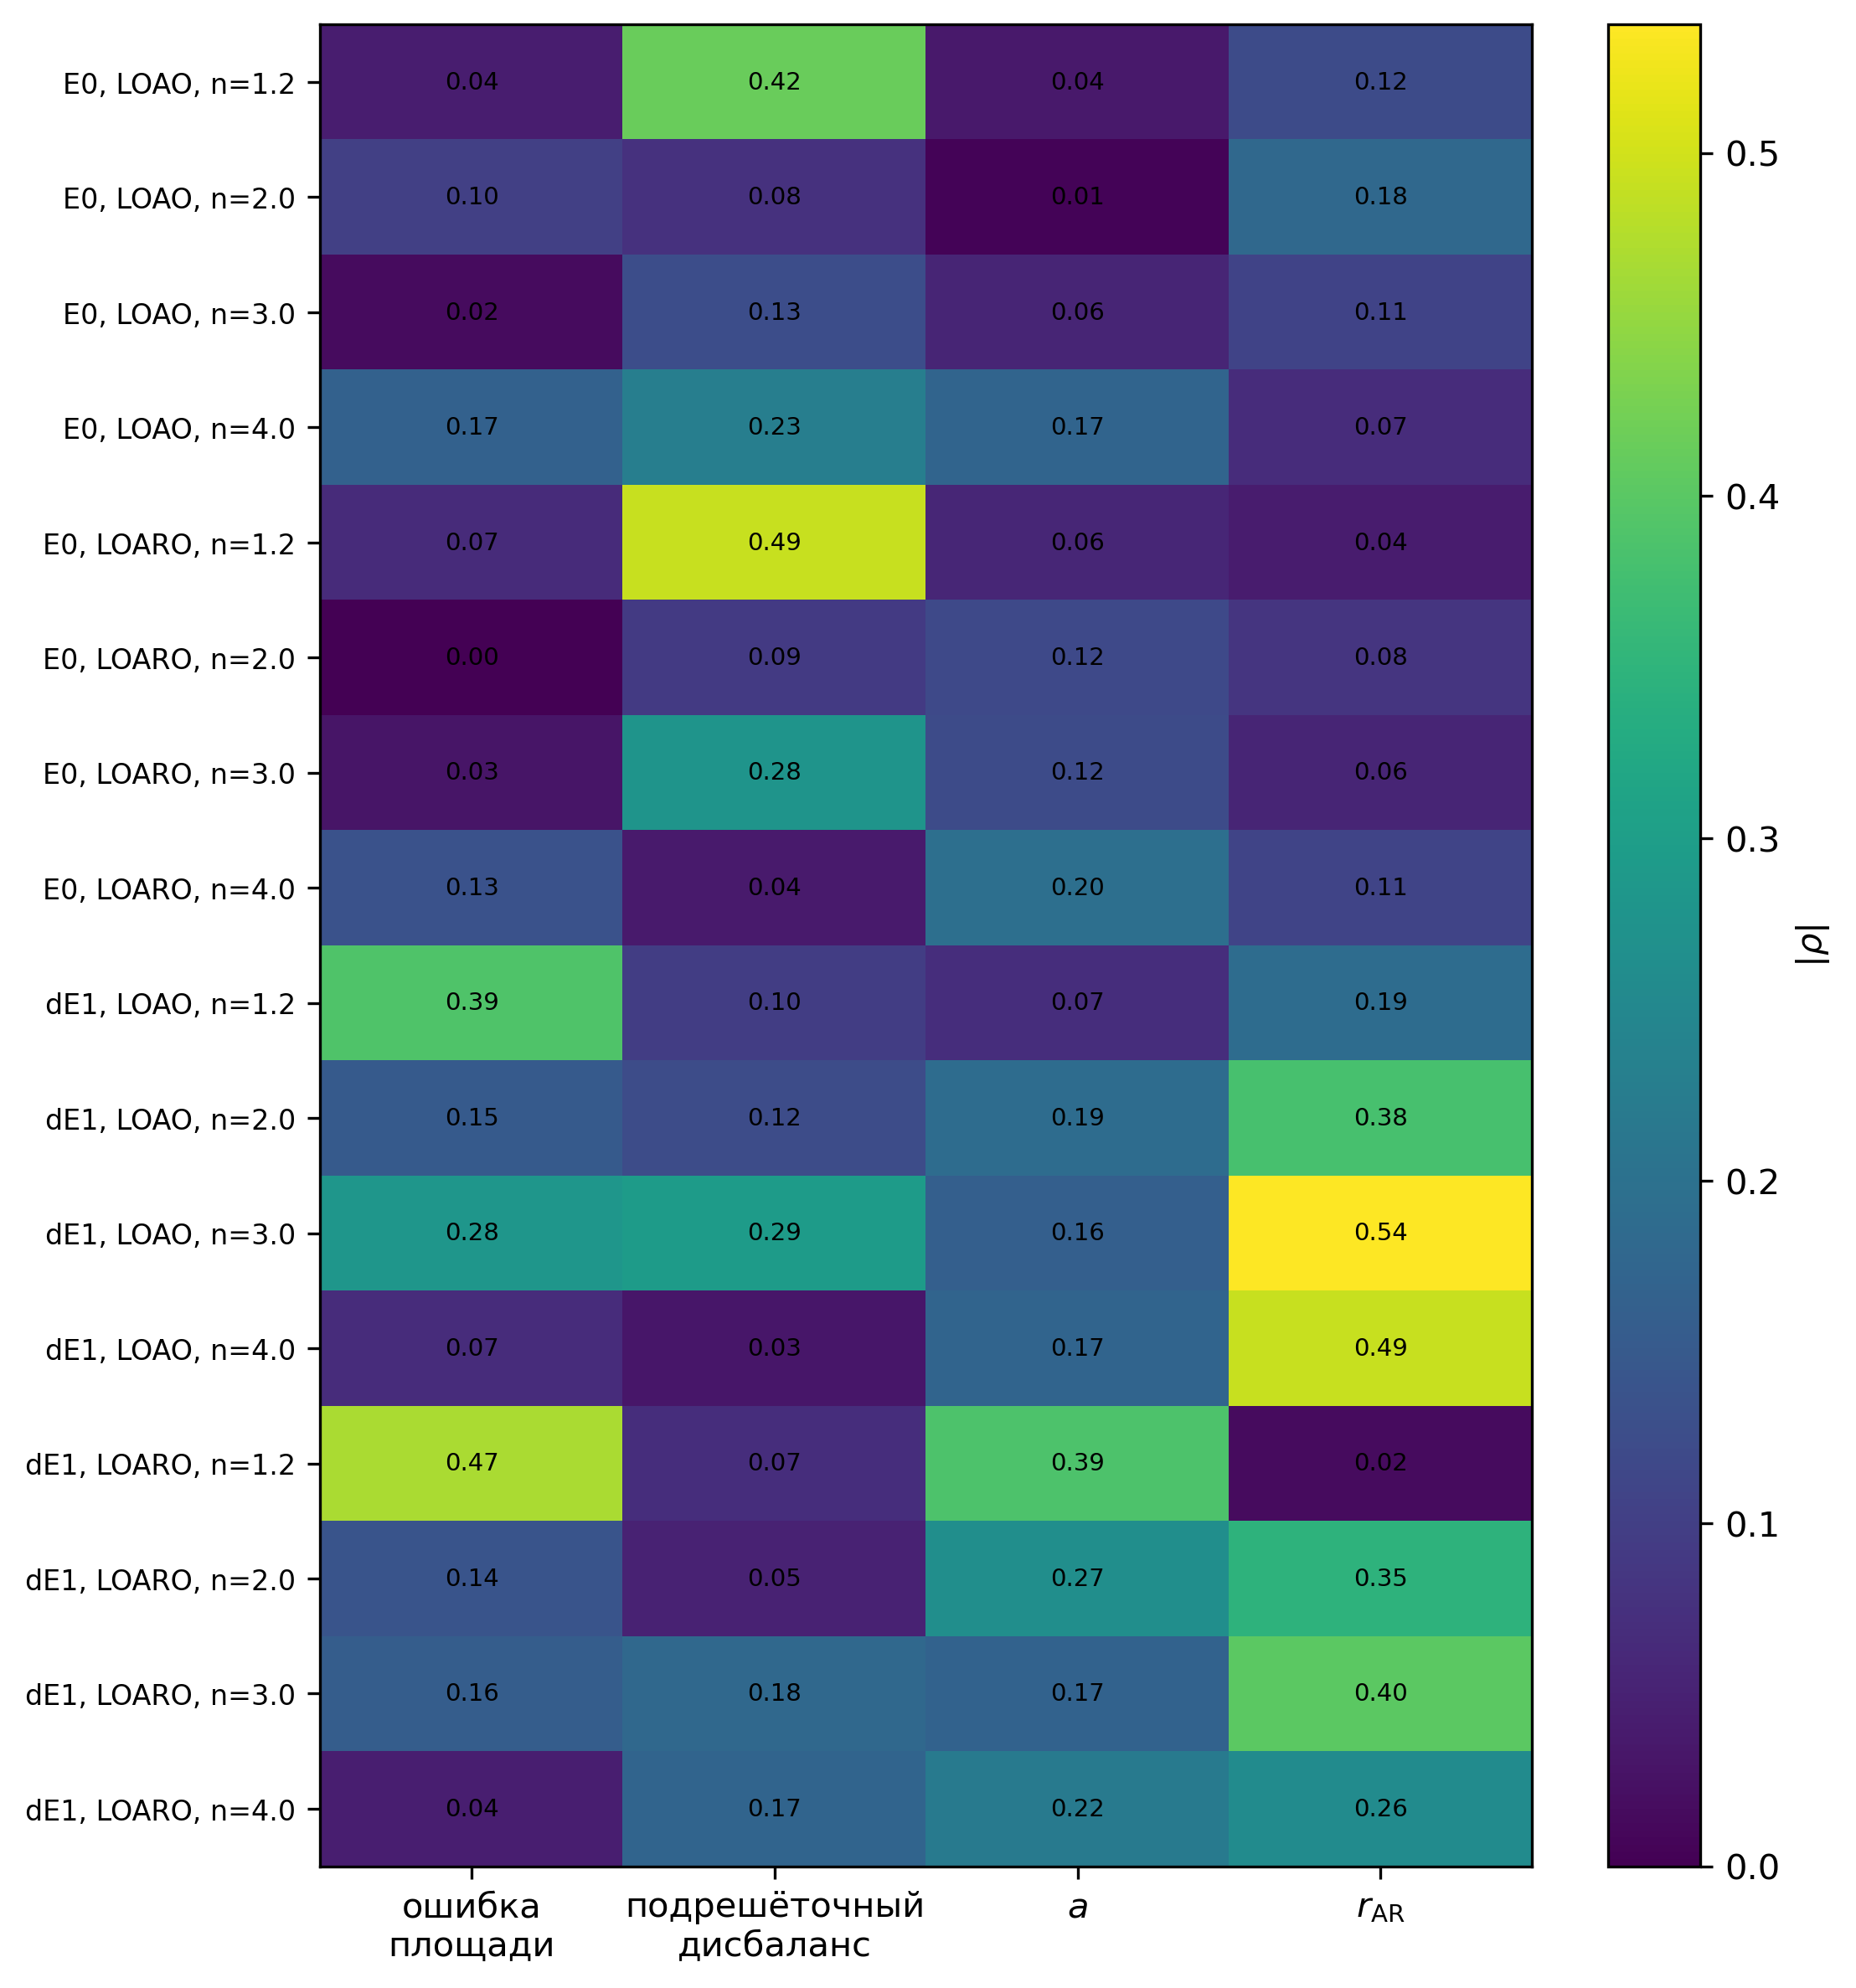
\includegraphics[width=0.85\textwidth]{../reports/assets/ridge_residual_correlation_heatmap.png}
  \caption{TODO: Карта корреляций остатков с диагностическими переменными.}
\end{figure}

\section{Проверяемый сценарий surrogate-assisted inverse screening}
\todo{This section is optional until step 10 is completed.}
\todo{Use Ridge only as a fast candidate filter.}
\todo{Validate all selected candidates by direct Kwant calculation.}
\todo{Do not present the surrogate as a substitute for direct Kwant validation.}
\todo{Stay inside the verified design window.}

\section{Ограничения применимости и связь с задачами нанодизайна}
\todo{Model is square-lattice TB, not material-specific DFT.}
\todo{No claim for arbitrary $n$.}
\todo{No claim for arbitrary shapes.}
\todo{No claim that MLP is unnecessary in all contexts.}
\todo{No claim that residuals are fully explained.}
\todo{Future work: DFT/OpenMX or material-specific TB calibration.}

\section{Выводы по главе 5}
\todo{Сформулировать выводы после завершения optional step 10 или явно отметить отсутствие inverse-screening результата.}

\clearpage

\chapter*{ЗАКЛЮЧЕНИЕ}
\addcontentsline{toc}{chapter}{ЗАКЛЮЧЕНИЕ}

\todo{Do not write the final conclusion yet. Replace this structured list after all results are frozen.}

\begin{enumerate}
  \item Confirm implementation and validation of Kwant/TB model.
  \item Confirm physical sanity checks.
  \item Confirm construction of fixed discrete-n superellipse dataset.
  \item Confirm Ridge as preferred surrogate.
  \item Confirm MLP ablation negative result under pre-registered criterion.
  \item Confirm residual analysis result and limitation.
  \item Optional inverse screening result if step 10 is completed.
  \item State future work: material-specific DFT/OpenMX calibration, larger datasets, other geometries, continuous-n models.
\end{enumerate}

\clearpage


\printbibliography[heading=bibintoc,title={СПИСОК ИСПОЛЬЗОВАННЫХ ИСТОЧНИКОВ}]

\appendix
\renewcommand{\thechapter}{А}
\setcounter{chapter}{1}
\setcounter{section}{0}
\clearpage
\begin{flushright}
\textbf{ПРИЛОЖЕНИЕ А}
\end{flushright}

\begin{center}
\textbf{Структура кода и воспроизводимость}
\end{center}

\vspace{0.8cm}
\addcontentsline{toc}{chapter}{Приложение А. Структура кода и воспроизводимость}

\section{Структура репозитория}

Репозиторий разделён на несколько функциональных частей. В каталоге \texttt{src/} находятся функции построения геометрий, формирования признаков и базовых моделей. Каталог \texttt{tests/} содержит автоматические проверки геометрических процедур, генерации данных и вспомогательных функций моделей. В \texttt{data/} размещены сохранённые расчётные массивы, используемые в главах с численными результатами. Каталог \texttt{notebooks/} содержит воспроизводимые расчётные блокноты для физических проверок, сравнения моделей и анализа остатков. В \texttt{reports/} сохранены итоговые таблицы и графики, а каталог \texttt{thesis/} содержит исходные файлы настоящего текста.

\section{Воспроизводимость}

Основная проверка программной части выполняется командой \texttt{conda run -n diplom-kwant python -m pytest tests -q}.

Расчётные блокноты воспроизводятся командой \texttt{jupyter nbconvert --to notebook --execute notebook.ipynb --inplace} для соответствующего файла из каталога \texttt{notebooks/}. Такой порядок отделяет прямой расчёт и анализ данных от текста дипломной работы: численные таблицы и рисунки сначала формируются в \texttt{reports/}, затем используются в \LaTeX{}-документе.

\section{Окружение}

Расчёты выполнялись в окружении \texttt{diplom-kwant}. Для воспроизведения требуются Python-библиотеки для численных расчётов, обработки таблиц, построения графиков, машинного обучения и работы с Kwant. В частности, численная линейная алгебра и стандартные процедуры машинного обучения опираются на общепринятые реализации SciPy и scikit-learn~\cite{virtanen2020scipy,pedregosa2011sklearn}. Конкретный набор зависимостей фиксируется проектными файлами и текущим окружением; перед повторным запуском расчётов необходимо активировать то же окружение или создать совместимое.

\section{Тесты}

Автоматические тесты проверяют корректность геометрических построений, согласованность формирования расчётных наборов и поведение функций базовых моделей. Отдельные проверки относятся к физически мотивированным признакам, конфигурации гребневой регрессии и многослойного перцептрона, а также к валидации входных параметров. Эти тесты не заменяют физические проверки из основной части работы, но уменьшают риск технических ошибок в расчётной процедуре.

\section{Сгенерированные расчётные блокноты и отчёты}

Итоговые численные материалы сформированы в блокнотах этапов 06c, 07, 08 и 09. Этап 07 создаёт таблицу физических проверок и рисунки масштабирования, круговой проверки, вырождения \(dE_2\) и дискретизационных диагностик. Этап 08 формирует таблицы сравнения гребневой регрессии и многослойного перцептрона, включая посеменную устойчивость и значения по группам исключения. Этап 09 сохраняет точечные остатки гребневой регрессии, корреляции с диагностическими величинами и сводку проверки гипотезы об остатках. Соответствующие CSV-таблицы и PNG-рисунки находятся в \texttt{reports/} и \texttt{reports/assets/}.

\clearpage

\chapter{ДОПОЛНИТЕЛЬНЫЕ ТАБЛИЦЫ}

\section{Расширенные fold-level результаты MLP}
\todo{Добавить выдержки или ссылки на reports/mlp_ablation_per_fold.csv.}

\section{Таблицы корреляций остатков}
\todo{Добавить выдержки или ссылки на reports/ridge_residual_correlations.csv и reports/ridge_residual_hypothesis_summary.csv.}

\section{Таблицы физических sanity checks}
\todo{Добавить выдержки или ссылки на reports/physics_sanity_checks.csv.}

\clearpage


\end{document}
